\documentclass{article}
\usepackage{listings} 
\usepackage{graphicx}
\usepackage{amsmath}
\usepackage{microtype}
\usepackage{hyperref}

% Global settings for listings
\lstset{
    basicstyle=\footnotesize\ttfamily, % Use a small typewriter font
    breaklines=true,                    % Automatic line breaking
    breakatwhitespace=false,            % Break lines not only at whitespace
    frame=single,                       % Frame around the code
    framesep=2pt,                       % Distance between frame and code
    framerule=0.5pt                     % Width of the frame
}

\newcommand{\HRule}[1]{\rule{\linewidth}{#1}}

\begin{document}

\title{ \normalsize \textsc{}
		\\ [2.0cm]
		\HRule{1.5pt} \\
		\LARGE \textbf{\uppercase{HIS Project - TSA}
		\HRule{2.0pt} \\ [0.6cm] \LARGE{Final Report} \vspace*{10\baselineskip}}
		}
\date{}
\author{\textbf{Author} \\ 
	Aneeq Ahmad - 1434617 \\
        Alberto Mejia - 1381799\\
        Jay Asodariya - 1439625\\
        Jemish Moradiya - 1417346\\
        Sidra Sarwar - 1417210\\
        Shrabanti Saha Rimi - 1377509
	}

\maketitle
\newpage

\tableofcontents
\newpage

\section{Chapter 01 Summary}

\subsection{Introduction}
This book serves as an advanced guide for data scientists and ML engineers to deepen their skills in time series analysis, a crucial and often overlooked aspect of ML. The book aims to progress beyond traditional methods such as ARIMA to the latest ML techniques, addressing the growing complexity and volume of business-related time series data.

\subsection{What is a Time Series?}
A time series is a sequence of observations recorded over time. Examples include the number of chocolate bars consumed over a month or monthly weight measurements. Time series can reveal relationships and trends, such as the correlation between chocolate consumption and weight changes, and can extend to other domains like stock prices and climate measurements.

\subsection{Types of Time Series}
The book distinguishes between regular time series with fixed time intervals and irregular ones without such consistency. Regular time series examples include hourly or monthly data points, while irregular ones could be patient lab test readings that occur sporadically.

\subsection{Applications of Time Series Analysis}
Three main applications are discussed: forecasting future values, classifying time series data (e.g., normal vs. abnormal EKG readings), and deriving causal inferences from time series to understand dynamics and relationships.

\subsection{Data-Generating Process (DGP)}
The DGP refers to the underlying mechanism that produces a time series, which is often stochastic and complex. Accurate forecasting hinges on closely approximating this DGP with a mathematical model.

\subsection{Synthetic Time Series Generation}
The book delves into generating synthetic time series by combining fundamental components such as noise and signals to simulate real-world data complexity. Techniques for creating white and red noise processes, cyclical or seasonal signals, and autoregressive signals are explained.

\subsection{Stationary vs. Non-Stationary Time Series}
Stationary time series have constant mean and variance over time, while non-stationary series display changes in these statistical properties due to trends or varying variance (heteroscedasticity), which complicates their analysis.

\subsection{Forecastability of Time Series}
Forecastability is dependent on understanding the DGP, the amount of historical data, and the presence of repeating patterns. The book categorizes time series predictability and discusses factors that influence it, such as the high predictability of tides compared to the randomness of lottery numbers or the volatility of stock prices.

\subsection{Forecasting Terminology}
The terminology section introduces concepts like multivariate forecasting, explanatory forecasting, backtesting, and forecast combination. It explains the role of in-sample and out-sample data, as well as exogenous and endogenous variables in the context of time series forecasting.

\subsection{Predicatbility}
The predictability of a time series is influenced by several factors:

\begin{itemize}
  \item \textbf{Understanding the Data-Generating Process (DGP):} A thorough understanding of the mechanisms that generate the time series data leads to better forecasting because the models can approximate the actual process more closely.
  \item \textbf{Amount of Data:} Access to a large volume of historical data improves predictability by revealing underlying trends, cycles, and variabilities.
  \item \textbf{Repeating Patterns:} Predictability is higher when the time series exhibits clear and consistent patterns that repeat over time.
  \item \textbf{Type of Data:} The inherent nature of the time series affects its predictability. Series influenced by well-understood phenomena (like tides) are more predictable than those with high randomness (like lottery numbers).
  \item \textbf{Statistical Characteristics:} The stationarity of a time series—constant mean, variance, and covariance—facilitates predictability. Non-stationary series are more challenging due to trends, seasonality, and other instabilities.
\end{itemize}

Each of these factors contributes to the overall predictability of a time series, with some series being inherently more predictable than others based on these characteristics.

\subsection{Forecasting}

\section{Chapter 01 Code Analysis}

\lstset{language=Python}
\begin{lstlisting}[frame=single]
    ar_value = [self.previous_value[i] * self.ar_param[i] for i in range(len(self.ar_param))]
    noise = np.random.normal(loc=0.0, scale=self.sigma, size=1)
    ar_value = np.sum(ar_value) + noise
    self.previous_value = self.previous_value[1:]+[ar_value[0]]
    return ar_value
\end{lstlisting}

\section{Chapter 02 Summary}

\subsection{Data Preprocessing}
Steps for Acquiring and Processing Time Series Data:

\section*{Steps to Acquiring and Processing Time Series Data}

\begin{enumerate}
    \item \textbf{Understanding the Time Series Dataset:} Gain insights into the structure, patterns, and characteristics of the time series data.
    
    \item \textbf{Preparing the Data Model:} Define the appropriate data model that suits the analysis objectives and ensures compatibility with the time series data.
    
    \item \textbf{Handling Missing Data:} Implement strategies to deal with missing values, including:
    \begin{enumerate}
        \item  {Last Observation Carried Forward (Forward Fill):} Replace missing values with the last observed value in the series.
        \item  {Next Observation Carried Backward (Backward Fill):} Replace missing values with the next observed value in the series.
        \item  {Mean Value Fill:} Replace missing values with the mean of neighboring values.
        \item  {Linear Interpolation:} Estimate missing values using linear interpolation between neighboring data points.
        \item  {Nearest Interpolation:} Estimate missing values using the value of the nearest available data point.
        \item  {Spline, Polynomial, and Other Interpolations:} Use more complex interpolation methods to estimate missing values based on the overall trend of the data.
    \end{enumerate}

       \item \textbf{Converting Data into Time Series Format:} Transform the data into time series format, considering:
    \begin{enumerate}
        \item  {Time Series Identifiers:} Define unique identifiers for each time series.
        \item  {Metadata or Static Features:} Include additional static information related to the time series.
        \item  {Time-Varying Features:} Extract features that vary over time and may influence the time series.
        \item  {Finding the Global End Date:} Determine the end date of the time series data to establish a common time frame.
        \item  {Basic Preprocessing:} Perform standard preprocessing steps such as normalization, scaling, or outlier removal.
        \item  {Mapping Additional Information:} Incorporate any supplementary data that can enhance the analysis or understanding of the time series.
    \end{enumerate}

    \item \textbf{Compact, expanded, and wide forms of data}
    \begin{enumerate}
        \item Wide (useless): We have the date as an index or as one of the columns and the different time series as different columns
        of the DataFrame. As the number of time series increases, they become wider and wider, hence the
        name.
        \item Expanded: is when the time series is expanded along the rows of a DataFrame. If there are
        n steps in the time series, it occupies n rows in the DataFrame.
        \item Compact: is when any particular time series occupies only a single row in the pandas
        DataFrame – that is, the time dimension is managed as an array within a DataFrame row.
    \end{enumerate}
    \item \textbf{Enforcing Regular Intervals in Time Series:} Ensure that the time series data follows a consistent and regular time interval, which is crucial for many time series analysis techniques.
        
    \item \textbf{Saving and Loading Files to Disk:} Save processed time series data to disk in an appropriate format for future use, and load data efficiently for analysis tasks.
\end{enumerate}

\subsection{Missing Data}

When dealing with longer periods of missing data in time series, various imputation techniques can be employed to fill in the gaps and maintain data continuity. Some commonly used methods include:

\begin{enumerate}
    \item \textbf{Imputing with the Previous Day:} Fill missing values by using the data from the preceding day. This method assumes that the data follows a similar pattern from one day to the next.
    
    \item \textbf{Hourly Average Profile:} Calculate the average values for each hour across the available data and use these averages to fill in the missing values for corresponding hours. This approach captures the typical behavior of the time series at different times of the day.
    
    \item \textbf{Hourly Average for Each Weekday:} Compute the average values for each hour of the day separately for each weekday (Monday, Tuesday, etc.). Then, use these weekday-specific averages to fill in missing values based on the day of the week. This method accounts for potential variations in patterns across different weekdays.
    
    \item \textbf{Seasonal Interpolation:} Estimate missing values by considering seasonal patterns in the data. This can involve fitting seasonal models, such as seasonal decomposition, and using the extracted seasonal components to interpolate missing values. Seasonal interpolation is particularly useful for time series data with recurring seasonal patterns.
\end{enumerate}

These techniques help maintain the integrity of the time series data when faced with longer periods of missing observations. The choice of method depends on the specific characteristics of the data and the underlying patterns that need to be preserved.

\section{Chapter 02 Code Analysis}
\begin{enumerate}
    \item Week of Year: {df.date.dt.isocalendar().week.iloc[0]} //error in reference to weekofyear
    \item Why add 4 days to the date range in line 22?
    \item Resampling is useful for aggregations and degradations
    \item Difference between y1=df.ISE and y2=df['ISE']?
    \item 
\end{enumerate}

This line should be skipped for the code to work
\lstset{language=Python}
\begin{lstlisting}[frame=single]
    df = df.loc["2022-07-07 7:00":"2022-07-07 09:00", "pm2_5_1_hr"]
    fig = px.line(df, x=df.index, y="pm2_5_1_hr", title="Missing Values in PM2.5")
    fig = format_plot(fig, ["Original"])
    fig.write_image("imgs/chapter_2/missing_values.png")
    fig.show()
\end{lstlisting}

There is a code error referencing the parent directory
\begin{lstlisting}[frame=single]
    os.makedirs("imgs/chapter_2", exist_ok=True)
    source_data = Path("scripts/data/london_smart_meters/") #scripts is added here
    block_data_path = source_data/"hhblock_dataset/hhblock_dataset"
    fig.show()
\end{lstlisting}


\section{Chapter 03 Summary}
Important topics discussed in chapter
\begin{enumerate}
    \item Components of a time series
    \item Visualizing time series data
    \item Decomposing a time series
    \item Detecting and treating outliers
\end{enumerate}

\subsection{Components of a Time Series}
The following terms can be mixed in different ways, but two very commonly assumed ways are additive and multiplicative
\begin{enumerate}
    \item Trend: is a long-term change in the mean of a time series. It is the smooth and steady movement of
    a time series in a particular direction.
    \item Seasonal: When a time series exhibits regular, repetitive, up-and-down fluctuations.
    \item Cyclical: is often confused with seasonality, but it stands apart due to a very subtle
    difference. Like seasonality, the cyclical component also exhibits a similar up-and-down pattern around
    the trend line, but instead of repeating the pattern every period, the cyclical component is irregular.
    \item Irregular: is left after removing the trends, seasonality, and cyclicity from a time series.
    Traditionally, this component is considered unpredictable and is also called the residual or error term. (Not completely useless. Can sometimes be explained by an exogenous varibale to a certain extent)
\end{enumerate}

\subsection{Visualizing Time Series Data}
\begin{enumerate}
    \item Line Charts 
    \item Seasonal (box)Plots 
    \item Calendar Heatmaps
    \item Autocorrelation plot
\end{enumerate}

\subsection{Decomposing a Time Series}
\subsubsection{Detrending}
Here we estimate the trend component (which is the smooth change in the time
series) and remove it from the time series, giving us a detrended time series.

Types:
\begin{enumerate}
    \item Moving averages: It can
    be seen as a window that is moved along the time series in steps, and at each step, the average of all
    the values in the window is recorded.
    \item Locally Estimated Scatterplot Smoothing (LOESS) Regression: We use an ordinal variable that moves between the time series as the independent
    variable and the time series signal as the dependent variable. For each value in the ordinal variable,
    the algorithm uses a fraction of the closest points and estimates a smoothed trend using only those
    points in a weighted regression. The weights in the weighted regression are the closest points to the
    point in question. This is given the highest weight and it decays as we move farther away from it. This
    gives us a very effective tool for modeling the smooth changes in the time series (trend).
\end{enumerate}

\subsubsection{Deseasonalizing}
Here, we estimate the seasonality component from the detrended time series.
After removing the seasonal component, what is left is the residual.

\begin{enumerate}
    \item Moving averages: It can
    be seen as a window that is moved along the time series in steps, and at each step, the average of all
    the values in the window is recorded.
    \item Fourier series: Any periodic function, no matter the shape, curve, or
    absence of it, or how wildly it oscillates around the axis, can be broken down into a series of sine and
    cosine waves.
\end{enumerate}

\subsection{Detecting and Treating Outliers}
An outlier, as its name suggests, is an observation that lies at an abnormal distance from
the rest of the observations. This can be for many reasons, including faulty measurement
equipment, incorrect data entry, and black-swan events, to name a few. Being able to detect such
outliers and treat them may help your forecasting model understand the data better.

Techniques:
\begin{enumerate}
    \item Standard Deviation
    \item Interquartile range
    \item Isolation Forest 
    \item Extreme studentized deviate (ESD) and seasonal ESD (S-ESD)
\end{enumerate}

\subsection{Decompositon}
Seasonal decomposition is the process by which we deconstruct a time series into its components 
typically, trend, seasonality, and residuals. The general approach for decomposing a time series is as follows:
\begin{itemize}
    \item Detrending: Here, we estimate the trend component (which is the smooth change in the time
series) and remove it from the time series, giving us a detrended time series.
    \item Deseasonalizing: Here, we estimate the seasonality component from the detrended time series.After removing the seasonal component, what is left is the residual.
\end{itemize}

\subsection{Outliers}
When treating outliers in time series data, it's crucial to determine whether correction is necessary. Automated outlier detection methods should be verified manually to avoid removing valuable patterns essential for forecasting. While it's feasible to inspect outliers in a few time series manually, for large datasets, automated techniques are preferred. Common practices include replacing outliers with heuristics like maximum, minimum, or percentiles. Alternatively, treating outliers as missing data and imputing them using established techniques is advisable. However, outlier correction might not be essential, especially with modern forecasting methods like machine learning or deep learning. The decision to correct outliers depends on experimentation and analysis of the specific dataset.

\section{Chapter 04}

\subsection{Setting up a test harness}

\subsubsection{Creating holdout (test) and validation dataset}

As a standard practice, in machine learning, we set aside two parts of the dataset, name them validation
data and test data, and don’t use them at all to train the model.

\begin{itemize}

    \item \textbf{validation set:} is used in the
    modeling process to assess the quality of the model. To select between different model classes, tune
    the hyperparameters, perform feature selection, and so on, we need a dataset.
    \item \textbf{holdout (test) set:} is like the final
    test of your chosen model. It tells you how well your model is doing in unseen data.

\end{itemize}

The best practice is to use the most recent part of the dataset as the test data. Additionally, it is advisable to have validation and test datasets of equal size to ensure that the decisions made during the modeling process, based on the validation data, are as applicable as possible to the test data.

\subsubsection{Chossing an evluation metric}
In time series forecasting
realm, there are scores of metrics with no real consensus on which ones to use. One of the reasons for
this overwhelming number of metrics is that no one metric measures every characteristic of a forecast.

\begin{itemize}
     \item \textbf{Mean Absolute Error (MAE):} Calculates the average absolute difference between actual and forecasted values, providing a measure of forecast accuracy that is robust to outliers.
    
    \item \textbf{Mean Squared Error (MSE):} Squares the differences between actual and forecasted values before averaging, giving more weight to large errors, making it sensitive to outliers.
    
    \item \textbf{Mean Absolute Scaled Error (MASE):} Compares the MAE of the forecast model with the MAE of a naive baseline model, providing a scaled measure of forecast accuracy that can be compared across different time series.
    
    \item \textbf{Forecast Bias (FB):} Measures the average tendency of the forecast to overpredict or underpredict, indicating if the forecast tends to be biased positively or negatively.

\end{itemize}

\subsection{Generating strong baseline forecasts}
Time series forecasting has been around since the early 1920s, and through the years, many brilliant
people have come up with different models, some statistical and some heuristic-based.

Refered to as:
\begin{itemize}
    \item \textbf{Naïve Forecast:} Assumes that the future value will be the same as the most recent observed value.
    \item \textbf{Moving Average Forecast:} Computes the average of the most recent observations, with the window size determining the number of observations included.
    \item \textbf{Seasonal Naive Forecast:} Similar to the naïve forecast, but considers the same seasonality period from the previous year.
    \item \textbf{Exponential Smoothing (ETS):} A family of forecasting methods that assigns exponentially decreasing weights to past observations.
    \item \textbf{Simple Exponential Smoothing (SES):} Updates forecasts based on a weighted average of past observations, with the weights declining exponentially.
    \item \textbf{Double Exponential Smoothing (DES):} Extends SES to account for trend by incorporating a second smoothing parameter.
    \item \textbf{Triple Exponential Smoothing or Holt-Winters (HW):} Incorporates seasonality in addition to trend and level components, making it suitable for seasonal data.
    \item \textbf{Autoregressive Integrated Moving Average (ARIMA):} A popular model that combines autoregression, differencing, and moving average components to capture time series patterns.
    \item \textbf{Theta Forecast:} A simplified version of ARIMA, primarily used for univariate time series forecasting.
    \item \textbf{Fast Fourier Transform Forecast:} Applies Fourier transform techniques to decompose time series data into its constituent frequencies, enabling forecasting based on periodic patterns.

\end{itemize}

After performing the aforementioned forecasting techniques it is important to remember that a comparison of their performance should be made. Not only concerning the forecast bias of each technique but also the time elapsed to perform the techniques.
When the 2-3 top candidates have finally been chosen, the forecasting algorithm can now be used on the validation and test data to assess which is the most adequate. 

\subsection{Assessing the forecastability of a time series}

Assessing the forecastability of a time series is crucial for determining the suitability of various forecasting models and techniques. Several metrics and measures can aid in this assessment:

\begin{enumerate}
    \item \textbf{Coefficient of Variation (CoV):} The CoV is the ratio of the standard deviation to the mean of the time series. It measures the relative variability of the data, with higher values indicating greater variability. A low CoV suggests a more predictable time series, whereas a high CoV may indicate higher uncertainty and complexity.
    
    \item \textbf{Residual Variability (RV):} RV quantifies the variance of the residuals obtained from a baseline forecast, such as a simple moving average or naive forecast. It provides insight into the level of unpredictability that remains after accounting for simple patterns in the data. Lower RV values indicate a more predictable time series.
    
    \item \textbf{Entropy-based Measures:} Entropy-based measures assess the randomness or disorderliness of a time series. Higher entropy values suggest greater disorder and unpredictability, while lower values indicate more regularity and predictability. Examples of entropy-based measures include Shannon entropy and approximate entropy.
    
    \item \textbf{Spectral Entropy:} Spectral entropy evaluates the distribution of spectral power across different frequencies in a time series. It measures the complexity of the frequency domain representation of the data, with higher values indicating greater complexity and unpredictability.
    
    \item \textbf{Kaboudan Metric:} The Kaboudan metric is a composite measure that combines various statistical properties of the time series, such as autocorrelation, skewness, and kurtosis, to assess forecastability. It provides a comprehensive evaluation of the time series characteristics and their impact on forecast performance.
\end{enumerate}

By analyzing these metrics, practitioners can gain insights into the underlying patterns, variability, and complexity of a time series, guiding the selection of appropriate forecasting models and strategies.

\section{Chapter 05 Summary}

\subsection{Understanding the basics of machine learning}
\subsubsection{Supervised machine learning tasks}
Machine learning can be used to solve a wide variety of tasks such as regression, classification, and recommendation. But, since classification and regression are the most popular classes of problems, we will spend just a little bit of time reviewing what they are.
\subsubsection{Overfitting and underfitting}
to machine learning models as well when they don’t learn enough patterns, and this is called underfitting.
Overfitting is an undesirable machine learning behavior that occurs when the machine learning model gives accurate predictions for training data but not for new data.
\subsubsection{Hyperparameters and validation sets}
Hyperparameters are parameters of the model that are not learned from data but rather are set before the start of training. For instance, the weight of the regularization is a hyperparameter.

\subsection{Time series forecasting as regression}
Time series forecasting, by definition, is an extrapolation problem, whereas regression, most of the time, is an interpolation one. Extrapolation is typically harder to solve using data-driven methods. Another key assumption in regression problems is that the samples used for training are \textbf{independent and identically distributed (IID).}. Thankfully, there are ways to convert a time series into a regression and
get over the IID assumption by introducing some memory to the machine learning model through
some features.

\subsubsection{Time delay embedding}
In time delay embedding, we assume a window of arbitrary length M < L and extract fixed-length subsequences from the time series by sliding the window over the length of the time series.
\subsubsection{Temporal embedding}
There are many ways to do this, from simply aligning a monotonically and uniformly increasing numerical column that captures the passage of time to sophisticated Fourier terms to capture the periodic components in time. 

\subsection{Local versus global models}
We can consider that all the time series in a related time series come from separate data generating processes (DGPs), and thereby model them all separately. We call these the local models of forecasting. An alternative to this approach is to assume that all the time series are coming from a single DGP. Instead of fitting a separate forecast function for each time series individually, we fit a single forecast function to all the related time series. This approach has been called global or cross- learning in literature.

\section{Chapter 06 Summary}

\subsection{Feature engineering}
Feature engineering, as the name suggests, is the process of engineering features from the data, mostly using domain knowledge, to make the learning process smoother and more efficient. 
Two main ideas to encode time into the regression framework: time delay embedding and temporal embedding.
\subsection{Avoiding data leakage}
Data leakage occurs when the model is trained with some information that would not be available at the time of prediction. Typically, this leads to high performance in the training set, but very poor performance in unseen data. There are two types of data leakage:
\begin{itemize}
    \item \textbf{Target leakage} is when the information about the target (that we are trying to predict) leaks into some of the features in the model
    \item \textbf{Train-test contamination} is when there is some information leaking between the train and test datasets.
\end{itemize}

\subsection{Setting a forecast horizon}
Forecast horizon is the number of time steps into the future we want to forecast at any point in time.

\subsection{Time delay embedding}
Time delay embedding is to embed time in terms of recent observations.
\begin{itemize}
    \item \textbf{Lags or backshift}
    \item \textbf{Rolling window aggregations}
    \item \textbf{Seasonal rolling window aggregations}
    \item \textbf{Exponentially weighted moving averages (EWMA)}
\end{itemize}


\subsection{Temporal embedding}
Temporal embedding as a process where we try to embed time into features that the ML model can leverage. 
\begin{itemize}
    \item \textbf{Calendar features}
    \item \textbf{Time elapsed}
    \item \textbf{Fourier terms}
\end{itemize}

\section{Chapter 07 Summary}

\subsection{Handling non-stationarity in time series}
Stationarity in econometrics assumes constant statistical properties over time. In time series and regression, this matters as we estimate a single function. For example, the number of park visitors pre- and post-pandemic illustrates concept drift, a phenomenon recognized in machine learning when a model's relevance shifts over time.


There are four main questions we can ask ourselves to check whether our time series is stationary or not:
\begin{itemize}
    \item Does the mean change over time? Or in other words, is there a trend in the time series?
    \item Does the variance change over time? Or in other words, is the time series heteroscedastic?
    \item   Does the time series exhibit periodic changes in mean? Or in other words, is there seasonality in the time series?
    \item     
    \item Does the time series have a unit root?
\end{itemize}

\subsection{Detecting and correcting for unit roots}
Time series analysis has its roots in econometrics and statistics and unit root is a concept derived directly from those fields.

\begin{itemize}
    \item \textbf{Unit roots}
    \item \textbf{The Augmented Dickey-Fuller (ADF) test}
    \item \textbf{Differencing transform}
\end{itemize}


\subsection{Detecting and correcting for trends}
In Chapter 5, we discussed time series forecasting as a challenging extrapolation problem, particularly due to trends. ARIMA and exponential smoothing address this by autoregression and explicit trend modeling. Standard regression may struggle with extrapolation, but with suitable features like lags, it becomes more adept. Detrending simplifies regression application by focusing on trend-removed data.
\begin{itemize}
    \item \textbf{Deterministic and stochastic trends}
    \item \textbf{Kendall’s Tau} is a measure of correlation but carried out on the ranks of the data. Similar to Spearman’s correlation, which also calculates correlation on ranked data, Kendall’s Tau is a non-parametric test and therefore does not make assumptions about the data. 
    \item \textbf{Mann-Kendall test (M-K test)} is used to check for the presence of a monotonic upward or downward trend. And since the M-K test is a non-parametric test, like Kendall’s Tau
    \item \textbf{Detrending transform}
\end{itemize}

\subsection{Detecting and correcting for seasonality}
\begin{itemize}
    \item \textbf{Detecting seasonality} autocorrelation function (ACF)
    \item \textbf{Deseasonalizing transform}
\end{itemize}
\subsection{Detecting and correcting for heteroscedasticity}
\begin{itemize}
    \item \textbf{Detecting heteroscedasticity}
    \item \textbf{Log transform}
    \item \textbf{Box-Cox transform}
\end{itemize}
\subsection{AutoML approach to target transformation}

\section{Chapter 07 Code Analysis}

Steps:
\begin{itemize}
    \item Preprocessed this file from chapter 6 is must 01-Feature Engineering.ipynb
\end{itemize}
Errors:
\begin{itemize}
	\item need to install joblib library
	\item need to install darts library for transformation models
    \item File Path error on each file path line

\end{itemize}

\section{Matlab for Time Series Analysis}
Example I have tried to run and understand on matlab
\begin{itemize}
    \item Find Events in Timetable Using Event Table
    \item Time Series Objects and Collections
\end{itemize}

\section{Chapter 08 Summary}
In the previous chapter, we introduced machine learning as a valuable tool for addressing time series forecasting problems. We discussed techniques such as time delay embedding and temporal embedding, which reframe time series forecasting as a classical regression task within the machine learning framework. In this chapter, we will delve deeper into these techniques, providing practical demonstrations using the London Smart Meters dataset that we have been exploring throughout this book.

The topics covered in this chapter include:

\begin{enumerate}
    \item Training and Predicting with Machine Learning Models:
    \begin{itemize}
        \item We will explore the process of training machine learning models for time series forecasting tasks. This involves preparing the data, selecting appropriate features, training the model, and making predictions.
    \end{itemize}
    
    \item Generating Single-Step Forecast Baselines:
    \begin{itemize}
        \item We will establish baseline performance metrics by generating single-step forecasts using simple algorithms or heuristics. These baselines will serve as benchmarks for evaluating the effectiveness of more advanced machine learning models.
    \end{itemize}
    
    \item Standardized Code for Training and Evaluating Machine Learning Models:
    \begin{itemize}
        \item We will provide standardized code snippets to streamline the process of training and evaluating machine learning models for time series forecasting. This will ensure consistency and reproducibility in our analyses.
    \end{itemize}
    
    \item Training and Predicting for Multiple Households:
    \begin{itemize}
        \item We will extend our analysis to handle time series data from multiple households within the London Smart Meters dataset. This will involve techniques for aggregating and processing data across multiple entities to create robust forecasting models.
    \end{itemize}
\end{enumerate}

By covering these topics, we aim to equip readers with the knowledge and practical skills necessary to leverage machine learning effectively for time series forecasting tasks, using real-world data from the London Smart Meters dataset as a case study.

\section{Training and Predicting with Machine Learning Models}

In Chapter 5, Time Series Forecasting as Regression, we discussed a schematic for supervised machine learning (Figure 5.2). In the schematic, we mentioned that the purpose of a supervised learning problem is to come up with a function, $\hat{y} = h(X, \phi)$, where $X$ is the set of features as the input, $\phi$ is the model parameters, and $h$ is the approximation of the ideal function. In this section, we are going to talk about $h$ in more detail and see how we can use different machine-learning models to estimate it.

$h$ is any function that approximates the ideal function, but it can be thought of as an element of all possible functions from a family of functions. More formally, we can say the following:
\[ \hat{y} = h(X, \phi), \quad \text{where} \ h \in \mathcal{H} \]
Here, $\mathcal{H}$ is a family of functions that we also call a model. For instance, linear regression is a type of model or a family of functions. For each value of the coefficients, the linear regression model gives you a different function and $\mathcal{H}$ becomes the set of all possible functions a linear regression model can produce.

There are many families of functions, or models, available. For a more complete understanding of the space, we will need to refer to machine learning books or resources. The Further reading section contains a few resources that may help you start the journey. As for the scope of this book, we narrowly define it as the application of machine learning models for forecasting, rather than machine learning in general. And although we can use any regression model, we will only review a few popular and useful ones for time series forecasting and see them in action. We leave it to you to strike out on your own and explore the other algorithms to become familiar with them as well. But before we look at the different models, we need to generate a few baselines again.

\section{Generating Single-Step Forecast Baselines}

In Chapter 4, we reviewed and generated baseline models for forecasting. However, due to the single-step forecasting requirement discussed in Chapter 6, we need to adjust our approach. Multi-step baseline models, such as ARIMA or ETS, require iterative fitting and prediction steps, which can be computationally expensive.

To address this, we have chosen the naïve method and seasonal naïve as baseline models for single-step forecasting. These methods are implemented using native pandas methods and serve as strong baselines due to their simplicity and effectiveness.

In the `chapter08` folder, there is a notebook named `00-Single Step Backtesting Baselines.ipynb`, which generates these baselines and saves them to disk. The notebook computes predictions, metrics, and aggregate metrics for both the validation and test datasets. The aggregate metrics for the test period are displayed in Figure 8.1.

To facilitate training and evaluation, a standard structure has been used consistently throughout the process. This structure ensures consistency and ease of understanding when working with the notebooks.

\section{Standardized Code to Train and Evaluate Machine Learning Models}

To ensure a standardized pipeline for training machine learning models, three configuration classes (FeatureConfig, MissingValueConfig, and ModelConfig) have been defined, along with a wrapper class (MLForecast) for scikit-learn-style estimators. Let's explore each of them:

\subsection{FeatureConfig}

$FeatureConfig is a Python dataclass defining key attributes and functions necessary for processing data. It includes parameters such as date, target, continuous_features, categorical_features, boolean_features, index_cols, and exogenous_features. Additionally, it provides a method called \texttt{get\_X\_y} to retrieve features and targets from a data frame.$

\subsection{MissingValueConfig}

This data class handles strategies for dealing with missing values. It includes parameters like \texttt{bfill\_columns}, \texttt{ffill\_columns}, and \texttt{zero\_fill\_columns}. The default strategy fills missing values with the column mean. The method \texttt{impute\_missing\_values} fills empty cells according to the specified strategy.

\subsection{ModelConfig}

ModelConfig holds details regarding the modeling process, including the choice of model, normalization, handling of missing values, and categorical encoding. It provides a method called \texttt{clone} to clone the estimator along with its configuration.

\subsection{MLForecast}

MLForecast is a wrapper class around scikit-learn-style models, utilizing the configurations defined above. It includes functions like \texttt{fit}, \texttt{predict}, and \texttt{feature\_importance} for training, predicting, and retrieving feature importance from the model, respectively.

\subsection{Helper Functions}

The provided notebook includes a helper function called \texttt{evaluate\_model} for evaluating different models. It standardizes the process of training, testing, and evaluating models, automating the process at scale.

The standardized implementation provided in this book serves as a starting point and guide for designing systems with your data.

\subsection{Regularization - A Geometric Perspective}
The sections provide a geometric interpretation of regularization techniques, focusing on the L1 and L2 norms used in Lasso (L1) and Ridge (L2) regression.

\subsection{Geometric Interpretation}
The L1 and L2 norms represent distances in n-dimensional space. L2 norm is the Euclidean distance while L1 norm is the Manhattan distance.

\subsection{Visual Representation}
In a city grid layout like Manhattan, L1 distance represents the actual distance a taxicab would travel between two points, while L2 distance represents the direct distance.

\subsection{Thought Experiment}
Moving a point in space while keeping L1 or L2 norm constant results in different shapes: a sphere for L2 and a diamond for L1.

\subsection{Optimization Perspective}
Regularization techniques like Lasso and Ridge regression encourage coefficients to stay within a defined distance from the origin, intersecting with the norm geometry.

\subsection{Sparse Solutions}
Lasso regression tends to produce sparse solutions by pushing some coefficients to zero, performing feature selection. Ridge regression shrinks coefficients towards zero but rarely to zero.

\subsection{Comparison and Implementation}
Demonstration of implementing and evaluating Ridge and Lasso regression models using Python's scikit-learn library.

\subsection{Transition to Decision Trees}
Discussion of decision trees, their ability to capture nonlinear relationships, susceptibility to overfitting, and strategies to mitigate it.

\section{Summary Figures}
The sections include figures illustrating the geometric interpretation of L1 and L2 norms, a comparison of regularization techniques, and feature importance in decision trees.

\section{Random Forest}
Ensemble learning combines multiple models to solve problems, leveraging the wisdom of the crowd concept. Bagging, a form of ensemble learning, uses bootstrap sampling to train weak learners and combines them through averaging or voting. Random Forest, proposed by Leo Breiman in 2001, modifies bagging by building a collection of decorrelated trees.

\subsection{Algorithm Overview}
In Random Forest, M trees are built. For each tree:
\begin{enumerate}
    \item Draw a bootstrap sample.
    \item Select random features.
    \item Split nodes using the selected features.
    \item Repeat until stopping criteria are met.
\end{enumerate}

\subsection{Prediction}
Prediction involves averaging (for regression) or majority voting (for classification) the outputs of all M trees.

\subsection{Implementation}
Hyperparameters like the number of trees and the number of features per split are crucial. Random Forest handles missing values and normalization differently from decision trees.

\subsection{Evaluation}
A sample forecast from RandomForestRegressor is shown, indicating room for hyperparameter tuning.

\section{Gradient Boosting Decision Trees}
Boosting combines weak learners sequentially. Gradient Boosting Decision Trees (GBDTs) use decision trees as weak learners.

\subsection{Algorithm Overview}
GBDTs build an additive ensemble of trees, optimizing each tree's contribution using gradients.

\subsection{Training Process}
The training process involves iteratively minimizing the loss function by adding trees.

\subsection{Regularization}
GBDTs are prone to overfitting and require regularization techniques. Parameters like learning rate and number of trees affect model complexity.

\subsection{Implementation}
Popular implementations include GradientBoostingRegressor in scikit-learn, XGBoost, LightGBM, and CatBoost.

\subsection{Evaluation}
A sample forecast from LightGBM is provided, demonstrating its superior performance.

\section{Summary}
The summary compares the performance of various machine learning models on a sample dataset, highlighting LightGBM as the top performer.

\section{Training and Predicting for Multiple Households}
We selected models (LassoCV, XGBRFRegressor, and LGBMRegressor) based on their performance metrics and runtime to run on all selected households in the validation dataset. The process involves looping over unique combinations, running different models, training, predicting, and evaluating. Aggregate metrics on all households in the validation dataset are shown in Figure 8.19.

\subsection{Aggregate Metrics}
Figure 8.19 illustrates that the models perform as expected even at the aggregated level, with predictions saved on disk.

\section{Using AutoStationaryTransformer}
In Chapter 6, AutoStationaryTransformer was applied to all households and the transformed dataset was saved. The process involved reading in transformed targets, joining them with the regular dataset, and defining FeatureConfig using the transformed target as the target and the original target as original_target.

\subsection{Notebook Check}
Notebooks 02-Forecasting with ML and Target Transformation and 02a-Forecasting with ML and Target Transformation for Test Dataset use transformed targets to generate forecasts for validation and test datasets, respectively. Summary metrics on transformed data are shown in Figure 8.21.

\subsection{Performance}
Figure 8.21 indicates that models using transformed targets don't perform as well as the original ones, possibly due to the dataset lacking strong trends.

\section{Conclusion}
This chapter provided practical training and evaluation of multiple models, enhancing understanding and skills in applying modern techniques to time series data. The next chapter will focus on combining forecasts and exploring concepts like combinatorial optimization and stacking for improved results.



\section{Chapter 09 Summary}
\subsection{Combining forecasts}

\subsection{Best fit}
This strategy of choosing the best forecast is by far the most popular and is as simple as choosing the best forecast for each time series based on the validation metrics. This strategy has been made popular by many automated forecasting software, which calls this the “best fit” forecast. The algorithm is very simple:
\begin{itemize}
    \item Find the best-performing forecast for each time series using a validation dataset.  
  	\item For each time series, select the forecast from the same model for the test dataset.
\end{itemize}


\subsection{Measures of central tendency}

\subsection{Simple hill climbing}
It is the simplest way to implement a hill climbing algorithm. It only evaluates the neighbor node state at a time and selects the first one which optimizes current cost and set it as a current state.

Few limitations of hill climbing
\begin{itemize}
    \item Runtime considerations
    \item Short-sightedness
    \item Forward-only
\end{itemize}

\subsection{Stochastic hill climbing}
The key difference between simple hill climbing and stochastic hill climbing is in the evaluation of candidates. In a simple hill-climb, we evaluate all possible options and pick the best among them. However, in a stochastic hill-climb, we randomly pick a candidate and add it to the solution if it is better than the current solution. This addition of stochasticity helps the optimization not get the local maxima/ minima. 

\subsection{Simulated annealing}
It is inspired by a physical phenomenon – annealing solids. Annealing is the process of heating a solid to a predetermined temperature (usually above its melting point), holding it for a while, and then slowly cooling it. This is done to ensure that the atoms assume a new globally minimum energy state, which induces desirable properties to some metals, such as iron.

\subsection{Optimal weighted ensemble}

\subsection{Stacking or blending}
We train another learning algorithm on the predictions of some base learners to combine these predictions. This second-level model is often called a stacked model or a meta model.
also known as \textbf{stacked generalization}

\textbf{Stacking} is when the meta model is trained on the entire training dataset, but with out-of-sample predictions.

\textbf{Blending} is similar to this but slightly different in the way we generate out-of-sample predictions.

\section{Chapter 10 Summary}

\subsection{Why Global Forecasting Models (GFMs)?}
The need for Global Forecasting Models (GFMs) in forecasting related time series datasets, highlighting shared attributes. Unlike Local Forecasting Models (LFMs), which treat each series independently, GFMs consider all series as originating from a single data generating process, offering more accurate and efficient forecasting. GFMs address drawbacks of LFMs, providing a holistic approach for improved modeling.
\begin{itemize}
     \item \textbf{Sample Size:}Stresses the importance of a large dataset for effective GFM training, ensuring a diverse and representative range of information.
     \item \textbf{Cross-learning:}Utilizes insights from one time series to improve forecasting for another, leveraging interdependencies between related series.
     \item \textbf{Multi-task learning:}Trains the GFM to handle multiple forecasting tasks simultaneously, capturing common patterns across different time series.
     \item \textbf{Engineering complexity:}Integrates complex features and relationships into the GFM for more nuanced and accurate forecasts.
\end{itemize}

\subsection{Creating GFMs}
Training Global Forecasting Models (GFMs) is straightforward by consolidating related time series into a single dataframe and training a unified model. It's crucial to ensure that all time series in the dataset have the same frequency to maintain performance. The standard framework from Chapter 8, used for Local Forecasting Models, can be adapted for GFMs. Specific adjustments, such as defining FeatureConfig and MissingValueConfig, are made in the notebook to accommodate the global modeling approach for all households in the London Smart Meters dataset.



\subsection{Strategies to improve GFMs}
\begin{itemize}
    \item \textbf{Increasing memory:}Enhances GFM performance by increasing memory capacity, allowing the model to capture longer-term dependencies in the time series
    \begin{itemize}
    \item \textbf{Adding more lag features:}Improves forecasting accuracy by incorporating lagged values of the target variable, capturing historical patterns.
    \item \textbf{Adding rolling features:}Boosts GFM's capability by introducing rolling statistics (e.g., rolling mean) to capture trends and changes in the time series over time.
    \item \textbf{Adding EWMA(Exponentially Weighted Moving Average ) features:}Introduces Exponentially Weighted Moving Average features, emphasizing recent observations in the time series for improved sensitivity to changes.
    \end{itemize}
    
    \item \textbf{Using time series meta-features:}Incorporates meta-features that provide additional information about the time series, enhancing the model's understanding of underlying patterns.
    \begin{itemize}
    \item \textbf{Ordinal encoding and one-hot encoding:}Transforms categorical variables into numerical representations (ordinal encoding) or binary vectors (one-hot encoding) for better model compatibility.
    \item \textbf{Frequency encoding:}Encodes categorical variables based on their frequency of occurrence, providing the model with information about the distribution of categories.
    \item \textbf{Target mean encoding:}Utilizes the mean of the target variable for different categories, enriching the model with information about the relationship between categorical features and the target.
    \end{itemize}
    \item \textbf{Tuning hyperparameters:}Optimizes GFM performance by fine-tuning hyperparameters through methods such as grid search, random search, or Bayesian optimization.
    \begin{itemize}
    \item \textbf{Grid search}
    \item \textbf{Random search}
    \item \textbf{Bayesian Optimization}
    \end{itemize}
    \item \textbf{Partitioning:}Divides the dataset into subsets for training and validation purposes, enhancing model robustness.
    \begin{itemize}
    \item \textbf{Random partitioning:}Splits the data randomly into training and validation sets.
    \item \textbf{Judgemental partitioning:}Divides the data based on domain knowledge or expert judgment.
    \item \textbf{Algorithmic partitioning:}Uses algorithmic methods to partition the data based on characteristics or patterns within the time series.
    \end{itemize}
    

\end{itemize}


\subsection{Bonus – interpretability}
Interpretability in the context of machine learning and artificial intelligence, defining it as the degree to which a human can understand the cause of a decision. Two approaches to interpretability are transparency, where the model is inherently simple and understandable, and post hoc interpretation, which involves techniques to understand model predictions. Post hoc techniques like permutation feature importance, Shapley values, and LIME are discussed as methods applicable to any machine learning model, including Global Forecasting Models (GFMs).

\section{Chapter 11 Summary}

\subsection{What is deep learning and why now?}

\begin{itemize}
    \item \textbf{Increase in compute availability}
    \item \textbf{Increase in data availability}
\end{itemize}

\subsection{Perceptron - The first neural network}
The Perceptron, developed by Frank Rosenblatt in the 1950s, is one of the first neural network models. It functions by taking weighted inputs, summing them, and then outputting a binary result based on a threshold. This model mimics the basic function of a biological neuron but is much simpler. Despite its simplicity and limitations (such as handling only linearly separable problems), the Perceptron laid the groundwork for more complex neural networks.

\begin{itemize}
    \item \textbf{Inputs:} These are the real-valued inputs that are fed to a Perceptron. This is like the dendrites in neurons that collect the input.
    \item \textbf{Weighted sum:} Each input is multiplied by a corresponding weight and summed up. The weights determine the importance of each input in determining the outcome.
    \item \textbf{Non-Linearity:} The weighted sum goes through a non-linear function.Real-world data is often complex and not linearly separable. A nonlinear function allows the neural network to capture and model these nonlinear relationships in the data. 
\end{itemize}


\subsection{Components of a deep learning system}
Deep learning is presented as a highly modular system, characterized by two key properties of its parametrized modules:

\begin{itemize}
    \item \textbf{Output production:} These modules can generate an output from a given input through a series of computational steps.
    \item \textbf{Feedback adjustment:} When provided with the desired output, the modules can communicate back to their inputs, indicating how they should change to more closely align with this desired outcome. This feedback mechanism helps in iteratively adjusting the inputs to reduce the difference between the actual and desired outputs.
\end{itemize}

The core of this concept is the use of differentiable functions, which is crucial for gradient-based optimization methods commonly employed in deep learning. This differentiability allows for efficient computation of gradients, which are used to update the parameters of the model in a direction that minimizes the error or loss. This makes deep learning models adaptable and effective for a wide range of complex tasks.

\subsection{Linear layers and activation functions}
Learns the best features by which we can make the problem linearly 
separable. Linearly separable means when we can separate the different classes (in a classification
problem) with a straight line.

\subsubsection{Linear Transformations (In hidden layers)}
\begin{itemize}
    \item \textbf{Purpose:} Linear transformations in neural networks are typically accomplished through operations like weighted sums. They are used to project input data into a different space.
    \item \textbf{Function:} A linear transformation combines input features in a linear way (e.g., summing up inputs each multiplied by their respective weights). This process is essential for feature combination and transformation.
    \item \textbf{Implementation and Impact:} Linear transformations alone cannot capture complex patterns in data, especially if the data is not linearly separable. They are limited to linear relationships.
\end{itemize}

\subsubsection{Intermediate Activation Functions (In hidden layers)}
\begin{itemize}
    \item \textbf{Purpose:} Activation functions introduce nonlinearity into the network. They help the network learn and represent more complex relationships in the data.
    \item \textbf{Function:} After the linear transformation, the activation function processes the result to produce a nonlinear output. Common activation functions include ReLU (Rectified Linear Unit), sigmoid, and tanh.
    \item \textbf{Implementation and Impact:} Without activation functions, a neural network, regardless of how many layers it has, would essentially be a linear regression model, unable to solve complex problems like image recognition or natural language processing.
\end{itemize}

Linear transformations handle the combination and re-scaling of input features, while activation functions introduce the necessary nonlinearity that allows the network to model complex patterns. A typical layer in a neural network sequentially applies a linear transformation followed by a nonlinear activation function. This combination enables the network to learn from and make predictions on complex, real-world data.

\subsubsection{Output Activation Functions (In output layer)}
\begin{itemize}
    \item \textbf{Purpose:} The output activation function is critical in adapting the final layer's output of a neural network to the format required for a specific task, such as regression, binary classification, or multiclass classification. It ensures that the network's output is interpretable and suitable for the problem at hand.
    \item \textbf{Function:} This function processes the output of the network's final linear transformation to produce a result that aligns with the nature of the target variable. For instance, in a binary classification task, it converts the final layer's output into a probability (between 0 and 1), while in a regression task, it might leave the output as is (linear activation) or apply a transformation to ensure the output falls within a certain range.
    \item \textbf{Implementation and Impact:} The selection and application of an output activation function have profound implications on the training dynamics, model accuracy, and result interpretability. It needs to be compatible with the loss function used, directly influencing how the model's performance is evaluated and optimized during training. This choice also determines how the final output is presented, making it crucial for ensuring the model's outputs are relevant and comprehensible for the given task.
\end{itemize}

\subsubsection{Loss function}
\begin{itemize}
    \item \textbf{Function:} A loss function, also known as a cost function, quantitatively measures how far the predictions of a neural network are from the actual target values. In mathematical terms, it calculates the error or difference between the predicted output and the true output. The specific form of a loss function can vary depending on the type of task. For example, Mean Squared Error (MSE) is common in regression tasks, while Cross-Entropy loss is often used in classification tasks.
    \item \textbf{Purpose:} The primary purpose of a loss function is to guide the training process of the neural network. By providing a quantifiable metric of how well the model is performing, the loss function becomes the objective that the training process aims to minimize. It serves as a feedback mechanism for the model, indicating how far off its predictions are, and thus how it needs to adjust its weights during training.
    \item \textbf{Implementation and Impact:} During training, the neural network uses an optimization algorithm, typically some form of gradient descent, to adjust its weights in a way that minimizes the loss function. The loss function must be compatible with the output activation function of the neural network. For instance, using a softmax activation in the output layer typically pairs with a cross-entropy loss function.
\end{itemize}

\subsection{Gradient descent}

\subsubsection{Forward Computation (Forward Propagation)}

\begin{itemize}
    \item This involves passing input data through the network, layer by layer, using the computations defined in each layer, to produce an output.
    \item The output is then compared to the desired output using a loss function to determine how close the model's prediction is to the actual target.
\end{itemize}

\subsubsection{Backward Computation (Backward Propagation)}
\begin{itemize}
    \item Once the output is obtained and the loss is calculated, this step involves computing the gradient of the loss function with respect to all the parameters in the network.
    \item The gradient, a generalization of derivatives for multivariate functions, indicates the rate of change of the loss with respect to changes in the network's parameters.
\end{itemize}

\subsubsection{Gradient and its Importance}
\begin{itemize}
    \item Gradients, akin to slopes in high school mathematics, inform us about the local slope of a function.
    \item By understanding the gradient of the loss function, gradient descent, a mathematical optimization technique, can be employed to adjust the network's parameters in a way that minimizes the loss, thus optimizing the model's performance.
\end{itemize}

\section{Chapter 12 Summary}

\subsection{Understanding the encoder-decoder paradigm}
The encoder-decoder algorithm is a fundamental architecture in deep learning, often used for sequence-to-sequence tasks. 
Its main purpose is to take a variable-length input sequence, encode it into a fixed-length representation (the encoder part), and then decode this representation into a variable-length output sequence (the decoder part).
In other words, it's used for tasks where you have an input sequence and want to generate a corresponding output sequence.
The encoder-decoder architecture allows deep learning models to handle input and output sequences of different lengths, making it powerful for tasks involving sequential data. 
It's particularly useful for tasks where the relationship between input and output is complex and not one-to-one.

\begin{itemize}
    \item \textbf{Input/Feature Space:} The input space, also known as the feature space, is where your original data resides. In the context of the encoder-decoder algorithm, the input space typically represents the data you're trying to process or transform.
    \item \textbf{Encoder:} The encoder takes the data from the input space and processes it layer by layer through neural networks.Each layer extracts increasingly abstract and meaningful features from the input data. 
    \item \textbf{Latent Space:} The output of the encoder is the latent representation in the latent space. This latent representation is a compressed, abstract, and semantically meaningful representation of the input data. It captures the essential information required for generating an appropriate output.
    \item \textbf{Decoder:} Takes this latent representation from the encoder and transforms it back into a form that corresponds to the output space. The decoder leverages the information encoded in the latent space to generate an appropriate output.
    \item \textbf{Loss:} Is a measure of how far the prediction is from the desired output. The goal in training the model is to minimize this loss. This training process ensures that the decoder learns to extract relevant information from the latent space and use it to generate accurate outputs.
\end{itemize}


\subsection{Feed-forward networks}
A Feed-forward network (FFN) or fully connected network is one of the simplest neural network architectures. 
It takes a fixed-size input vector and processes it through a series of layers to produce the desired output. 
The term "feed-forward" signifies that data flows in one direction through the network, and "fully connected" means that each unit in a layer is connected to every unit in the previous and subsequent layers.

\begin{itemize}
    \item \textbf{Input and Output Layers:} The first layer is called the input layer, and its size matches the dimension of the input data. The final layer is the output layer, which is determined by the desired output format. For example, if you need one output, you have one unit in the output layer; if you need ten outputs, you have ten units.
    \item \textbf{Hidden Layers:} All the layers between the input and output layers are known as hidden layers. These layers contain units that perform computations and contribute to the network's ability to learn complex patterns.
    \item \textbf{Network Structure:} The structure of the FFN is defined by two key hyperparameters: the number of hidden layers and the number of units in each layer. These hyperparameters determine the network's capacity to represent and learn from the data.
\end{itemize}

In the context of time series forecasting, an FFN can serve as both an encoder and a decoder. 
As an encoder, it can transform time series data, making it suitable for regression tasks. 
As a decoder, it operates on the latent vector, generated by the encoder, to produce the desired output. 
This decoder role is the most common use of FFNs in time series forecasting.

\subsection{Recurrent neural networks}
RNNs are a class of neural networks specifically designed for processing sequential data. 
They are particularly well-suited for tasks where the order and context of the data matter. 
Unlike feed-forward networks (FFNs), RNNs have connections that loop back on themselves, allowing them to maintain a hidden state, or memory, that captures information from previous timesteps.

Key Components of an RNN:
\begin{itemize}
    \item \textbf{Hidden State (Memory):} The core component of an RNN is the hidden state, often referred to as the "memory." It's a vector that stores information about the data seen in previous timesteps. This hidden state is updated at each timestep based on the current input and the previous hidden state.
    \item \textbf{Input:} At each timestep, the RNN receives an input, which could be a single element of a sequence or a vector representing the entire input at that timestep. The input is used to update the hidden state.
\end{itemize}

In essence, Recurrent Neural Networks (RNNs) can be conceptualized as comprising two concurrent feed-forward networks (FFNs). 
The first FFN operates on the input data, mapping it to a specific output. 
Simultaneously, the second FFN is applied to the initial hidden state, aiming to transform it into a specific hidden state output.
As a result, RNN blocks can be organized to accommodate a diverse range of input and output scenarios, including many-to-one setups, as well as many-to-many configurations.
That being said, the main drawback of RNNs in sequence modeling is the potential for vanishing or exploding gradients during backpropagation, which occurs as the network struggles with lengthy sequences, leading to either halted learning or unstable training.
We can analogize this phenomenon to the process of repeatedly multiplying a scalar number by itself: If the number is less than one, it gradually diminishes with each iteration, approaching zero; conversely, if the number exceeds one, it rapidly grows exponentially.


\subsection{Long short-term memory (LSTM) networks}
LSTM was designed to address the challenges of vanishing and exploding gradients encountered in vanilla RNNs. 
The core concept behind LSTM is inspired by computer logic gates, and it introduces a crucial element known as a "memory cell" to facilitate long-term memory retention alongside the traditional hidden state memory of RNNs.

\begin{itemize}
    \item \textbf{Input Gate:} This gate determines how much information to read from the current input and the previous hidden state.
    \item \textbf{Forget Gate:} The forget gate's role is to decide how much information should be discarded from the long-term memory.
    \item \textbf{Output Gate:} The output gate determines the extent to which the current cell state contributes to creating the current hidden state, which serves as the output of the cell.
    \item \textbf{Memory Cell:} It can be thought of as a container that holds information over multiple timesteps. It has the capability to store and update information for long-term dependencies, and its content is modified by the input and output gates.
\end{itemize}

So, while both RNNs and LSTMs have elements that can be seen as forms of memory, the memory cell in LSTMs is a more specialized and flexible mechanism explicitly designed to address the limitations of traditional RNNs in capturing and retaining long-term information in sequential data.

\subsection{Gated recurrent unit (GRU)}
The idea behind GRU is akin to using gates to control the flow of information within the network. 
However, GRU distinguishes itself by eliminating the long-term memory cell component found in LSTMs. 
Instead, it relies solely on the hidden state to convey and manage information. 
In essence, the hidden state itself acts as the "gradient highway," enabling information to pass through the network efficiently. 
Unlike LSTMs, GRUs use two key gates: the reset gate, which determines how much of the previous hidden state is considered when computing the candidate's hidden state for the current timestep, and the update gate, which governs how much of the previous hidden state is carried forward and how much of the current candidate's hidden state contributes to the new hidden state.

In relation to the previously mentioned concepts, GRUs are another variation of recurrent neural networks designed to address the challenges faced by traditional RNNs. 
Similar to LSTMs, GRUs introduce gating mechanisms to control information flow, but they simplify the architecture by eliminating the dedicated memory cell. 
Instead, GRUs rely on the hidden state as the primary carrier of information, making them computationally more efficient and suitable for capturing dependencies in sequential data.


\subsection{Convolution networks}
At the core of CNNs lies the mathematical operation of convolution, which plays a central role in data processing. 
In the context of image data, CNNs employ kernels, which are 2D matrices with numerical values. 
These kernels are smaller than the images they operate on, and they are "slid" across the image, performing element-wise multiplications and summations at each position. 
This process allows CNNs to extract features from the data effectively.

For time series data, CNNs transition to 1D convolutions, where a 1D kernel is similarly moved along the sequence to produce an output. 
Unlike manually engineered features, CNNs learn the kernel weights from the data, making them adaptable and capable of generating various features. 
By adjusting kernel weights, CNNs can capture different characteristics in the data, enhancing their capacity as feature generators.

1D Convolution for Time Series Data:
\begin{itemize}
    \item \textbf{Kernel Movement:} Similar to image data, 1D kernels are moved along the sequence of data points. At each position, the kernel interacts with a segment of the time series data, performing element-wise operations and producing an output value.
    \item \textbf{Learnable Weights:} Just like with image data, the weights within the 1D kernels are learned from the time series data during training. This adaptability enables CNNs to discover meaningful patterns or features in the sequence.
    \item \textbf{Feature Generation:} By adjusting the weights within the kernels, CNNs can capture different characteristics within the time series. For example, specific weights may emphasize short-term trends, while others may focus on long-term patterns. This flexibility makes CNNs powerful feature generators for time series analysis.
    \item \textbf{Adaptive Learning:} It's crucial to note that the values within these kernels are not fixed but are learned by the CNN during training. This adaptability allows CNNs to adjust their feature extraction behavior based on the specific dataset and task.
    \item \textbf{Stride:} refers to the step size at which a convolutional kernel moves across the input data during the convolution operation. It determines how much the kernel "jumps" or shifts between each operation.
    \item \textbf{Dilation:} Adjusts the gaps or "holes" between the kernel values during convolution, expanding the receptive field without changing the kernel size, enabling the layer to capture more input information.
    \item \textbf{Receptive Field:} The receptive field of a convolutional layer is the area in the input data that influences the feature generated by that layer. It's essentially the spatial extent or size of the input window over which the convolution operation is performed.
\end{itemize}

It it important to note that in multi-layered Convolutional Neural Networks (CNNs), calculating the receptive field becomes more complex due to the hierarchical structure of the network.
In multi-layered CNNs, each layer processes features extracted by previous layers. As a result, the receptive field of deeper layers encompasses larger portions of the input data, allowing them to capture more context and complex patterns.

\section{Chapter 13 Summary}

\subsection{Tabular regression}
Tabular regression in time series forecasting involves using structured data arranged in rows and columns to predict future values. This approach applies regression models, such as linear regression or decision trees, to learn patterns from historical data, considering features like past values and external factors. The process includes data preparation, feature engineering, model training, evaluation, and making predictions. The effectiveness depends on the chosen algorithm and the characteristics of the time series data.

\subsection{Single-step-ahead recurrent neural networks}
Single-step-ahead recurrent neural networks (RNNs) are designed for time series forecasting, predicting the next value in a sequence based on previous values. They use recurrent connections to maintain a memory of past inputs. During training, the model learns patterns in historical data, and after training, it can predict the next value given a sequence of past values. Advanced variants like LSTM and GRU address some limitations of basic RNNs.

\subsection{Sequence-to-sequence models}
Sequence-to-sequence (Seq2Seq) models are neural networks designed for tasks like language translation and summarization. They consist of an encoder to process input sequences and a decoder to generate output sequences. Attention mechanisms enhance their ability to handle varying-length sequences, making them valuable for tasks with diverse structures.
\subsubsection{RNN-to-fully connected network}
Combining an RNN with a fully connected network involves using an RNN to capture sequential patterns and connecting its output to a fully connected layer for further processing or classification. This hybrid architecture is useful for tasks where both sequential and global information are relevant.
\subsubsection{RNN-to-RNN}
Connecting one RNN to another, often termed "stacking" or "chaining" RNNs, allows for capturing more complex dependencies in sequential data. This is common in tasks where hierarchical or long-range dependencies are crucial. Each RNN layer processes information sequentially before passing it to the next layer.

\subsection{Summary}
In the previous chapter, we applied basic deep learning concepts using PyTorch for common modeling patterns. We explored RNN, LSTM, and GRU for time series prediction, then delved into Seq2Seq models, combining encoders and decoders. Encoders and decoders can be complex, even mixing convolution and LSTM blocks. We introduced "teacher forcing" for faster training and improved performance. In the next chapter, we'll dive into the popular and attention-grabbing topic of attention and transformers.

\section{Chapter 14 Summary}

\subsection{Convolutional Neural Network (CNN)}
CNNs play a crucial role in various applications, particularly in computer vision, due to their ability to automatically learn hierarchical features from input data.
\begin{itemize}
    \item \textbf{Feature Extraction} automatically extracting hierarchical features from input data. Through a series of convolutional and pooling layers, they learn to recognize low-level features like edges and textures, which progressively combine to form more complex and abstract features\cite{r1}.
    \item \textbf{Spatial Hierarchies}  helps in building a robust representation of the input.
    \item \textbf{Translation Invariance} meaning they can recognize patterns regardless of their position in the input. 
    \item \textbf{Transfer Learning} involves taking a pre-trained CNN and fine-tuning it on a specific dataset, often resulting in improved performance with less training data.
    \item \textbf{Texture and Pattern Recognition} recognizing textures and patterns in data, making them valuable in tasks where local patterns and structures are essential, such as medical imaging and satellite image analysis\cite{r2}.
    \item \textbf{Reduced Parameter Sharing} significantly reduces the number of parameters compared to fully connected networks. This parameter efficiency makes CNNs computationally feasible for large-scale image datasets.
\end{itemize}

\subsection{Combinations}
Main ways to combine a convolutional neural network (CNN) and a long short-term memory (LSTM) network:

\begin{itemize}
    \item Use the output of the CNN as the input to the LSTM. This allows the LSTM to learn features from the input data that have been learned by the CNN.
    \item Use the output of the LSTM as the input to the CNN. This allows the CNN to learn features from the output of the LSTM.
    \item Use a parallel architecture, where the CNN and LSTM operate on the input data independently, and their outputs are concatenated and passed to the fully connected layer.
\end{itemize}

\subsection{Classification and forecasting solutions}
\subsubsection{Classification}
\begin{itemize}
    \item \textbf{Image Classification}  learn hierarchical features from images and can automatically extract patterns and shapes. Architectures like AlexNet, VGGNet, and ResNet have been successful in various image classification challenges\cite{r3}.
    \item \textbf{Transfer Learning for Classification} often leads to improved performance, especially when labeled data is limited.
    \item \textbf{Spatial Hierarchies in Time Series Data} can be adapted for classification. Each time step becomes a pixel in the "image," and the CNN learns spatial hierarchies of features over time.
\end{itemize}

\subsubsection{Forecasting}
\begin{itemize}
    \item \textbf{1D CNNs for Time Series} can be used for time series data. The operation is applied along the temporal axis, capturing local patterns and dependencies.
    \item \textbf{Temporal Convolution} learns filters that can identify relevant features over different time scales, making them suitable for forecasting tasks.
    \item \textbf{Hybrid Models} combining CNNs with recurrent neural networks (RNNs) or long short-term memory networks (LSTMs) are increasingly used for time series forecasting. CNNs can capture local patterns, while RNNs or LSTMs can model temporal dependencies.\cite{r4}
    \item \textbf{Multivariate Time Series} network can learn patterns and relationships between different variables, enhancing forecasting capabilities.
    \item \textbf{Feature Learning} powerful feature extractors, automatically learn relevant features from the input data, reducing the need for manual feature engineering.
\end{itemize}

\subsection{What is attention?}
In deep learning, attention is a mechanism inspired by human cognitive function. It allows neural networks to dynamically focus on specific parts of input sequences, emphasizing relevant information while de-emphasizing less important parts. This attention mechanism is particularly useful in tasks involving sequences, such as natural language processing and time series analysis. It enables models to weigh different parts of the input sequence differently, enhancing their ability to capture complex relationships and dependencies.
\subsection{Generalized attention model}
A generalized attention model is a flexible extension of the traditional attention mechanism in deep learning. It allows for customization in how attention is computed and applied, providing adaptability for different tasks and data characteristics. It enables neural networks to dynamically focus on specific parts of input sequences, enhancing their ability to capture complex relationships and dependencies.
\subsubsection{Alignment functions}
There are many variations of the alignment function that have come up over the years. Let’s review a
few popular ones that are used today.
\begin{itemize}
    \item \textbf{Dot product:} Simplest alignment function. Measures similarity by taking the dot product of query and key vectors. Requires the same dimensions for query and key vectors.
    \item \textbf{Scaled dot product attention:} Variation of the dot product with scaling to control the magnitude of the gradients. Mitigates issues with vanishing or exploding gradients.
    \item \textbf{General attention:} Allows for different weight matrices for query and key vectors. Adds flexibility compared to dot product attention.
    \item \textbf{Additive/concat attention:} Combines query and key vectors through concatenation followed by a trainable matrix. Introduces non-linearity, enhancing expressive power. Offers another level of flexibility in modeling attention.

\end{itemize}

\subsubsection{Distribution function}
The distribution function's main purpose is to convert learned scores from the alignment function into weights that sum up to 1. The widely used softmax function accomplishes this, interpreting weights as probabilities. However, softmax has drawbacks, as it assigns some weight to every element, lacking sparsity. Alternatives like sparsemax and entmax address this by allowing probability mass on select relevant elements and assigning zero to others. These functions are useful when knowledge encoding involves only a few timesteps, enhancing interpretability and avoiding implausible options.
\subsection{Forecasting with sequence-to-sequence models and attention}
Forecasting with Seq2Seq models and attention involves using neural networks designed for sequential data. The encoder processes historical data, and attention helps the decoder focus on specific information during sequence generation. This approach improves accuracy by capturing complex patterns and dependencies, making it valuable for various forecasting tasks like stock prices or weather predictions.
\subsection{Transformers – Attention is all you need}
"Attention Is All You Need" (2017) introduced Transformers, a revolutionary architecture using scaled dot product attention, discarding recurrent networks for more efficiency in processing long sequences. Transformers, highlighted by BERT in 2018, dominate NLP, time series forecasting, reinforcement learning, and computer vision tasks. The original 2017 Transformer architecture remains foundational amid numerous adaptations.
\subsubsection{Key component of Transformer model}
\begin{itemize}
    \item \textbf{Self-attention: }Allows each word in a sequence to focus on other words, capturing relationships and dependencies efficiently.
    \item \textbf{Multi-headed attention: }Utilizes multiple self-attention mechanisms in parallel, providing the model with diverse perspectives on relationships within the sequence.
    \item \textbf{Positional encoding: }Incorporates position information into the input embedding, addressing the model's lack of inherent understanding of sequence order.
    \item \textbf{Position-wise feed-forward layer: }Applies a feed-forward network independently to each position in the sequence, enhancing the model's ability to capture different features.
\end{itemize}

\subsubsection{How the component put together}
\begin{itemize}
    \item \textbf{Encoder: }The vanilla Transformer model is an encoder-decoder model. There are N blocks of encoders, and each block contains an MHA layer and a position-wise feed-forward layer with residual connections in between.
    \subitem \textbf{Residual connections: }Introduces shortcut connections that help mitigate the vanishing gradient problem during training.
    \subitem \textbf{Layer normalization: }Normalizes input to each layer, stabilizing training by reducing internal covariate shift.
    \item \textbf{Decoder: }The decoder block is also very similar to the encoder block, but with one key addition. Instead of a single self-attention layer, the decoder block has a self-attention layer, which operates on the decoder input, and an encoder-decoder attention layer.  
    \subitem \textbf{Masked self-attention: }Allows each position to attend to all positions in the decoder up to and including that position, preventing information leakage from future positions.
\end{itemize}

\subsection{Forecasting with Transformers}
Forecasting with Transformers involves using the Transformer architecture for time series prediction. The self-attention mechanism enables the model to capture complex dependencies, and positional encoding addresses sequence order. Trained on historical data, Transformers excel in handling long-range dependencies, making them effective for various forecasting tasks, including stock prices and weather predictions.


\subsection{Understanding the encoder-decoder paradigm}
Deep learning, including the encoder-decoder paradigm, is employed in time series analysis to learn patterns from historical data for future predictions. In 1997, Ramon Neco and Mikel Forcada proposed an architecture for machine translation that had ideas reminiscent of the encoder-decoder paradigm. In 2013, Nal Kalchbrenner and Phil Blunsom proposed an encoder-decoder model for machine translation, although they did not call it that. The encoder-decoder architecture, pioneered around 2014 by Cho et al. and Sutskever et al., enables modeling variable-length inputs and outputs, facilitating end-to-end learning for tasks like machine translation.

The feature space, or the input space, is the vector space where your data resides. If the data has 10 dimensions, then the input space is the 10-dimensional vector space. Latent space is an abstract vector space that encodes a meaningful internal representation of the feature space. To understand this, we can think about how we, as humans, recognize a tiger. We do not remember every minute detail of a tiger; we just have a general idea of what a tiger looks like and its prominent features, such as its stripes. It is a compressed understanding of this concept that helps our brain process and recognize a tiger faster.

Now that we have an idea about latent spaces, let’s see what an encoder-decoder architecture does. An encoder-decoder architecture has two main parts: an encoder and a decoder.
\begin{itemize}
    \item \textbf{Encoder: } The encoder takes in the input vector, x, and encodes it into a latent space. This encoded representation is called the latent vector, z.
    \item \textbf{Decoder: } The decoder takes in the latent vector, z, and decodes it into the kind of output we need $(y\hat{y})$.

\end{itemize}

\begin{center}
    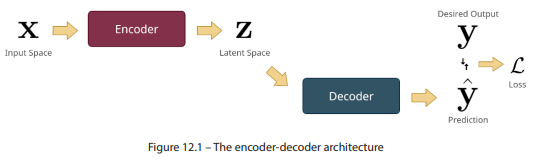
\includegraphics[width=.5\textwidth]{Picture1.png}
\end{center}

In the context of time series forecasting, the encoder consumes the history and retains the information that is required for the decoder to generate the forecast. As we learned previously, time series forecasting can be written as follows: 

\begin{center}
    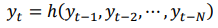
\includegraphics[width=.5\textwidth]{Picture2.png}
\end{center}

Now, using the encoder-decoder paradigm, we can rewrite it as follows:

\begin{center}
    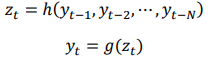
\includegraphics[width=.5\textwidth]{Picture3.png}
\end{center}

Here, h is the encoder and g is the decoder.
Each encoder and decoder can be some special architecture suited for time series forecasting. Let’s look at a few common components that are used in the encoder-decoder paradigm.

\subsubsection{Feed-forward networks}
Feed-forward networks (FFNs) or fully connected networks are the most basic architecture a neural network can take. We discussed perceptrons in Chapter 11, Introduction to Deep Learning. If we stack multiple perceptrons (both linear units and non-linear activations) and create a network of such units, we get what we call an FFN.

A Feedforward Neural Network (FFN) processes a fixed-size input vector through computational layers, culminating in the desired output. It's termed "feed-forward" because information moves sequentially through the network. Also known as a fully connected network, each unit in a layer connects to every unit in the previous and next layers. The input layer matches the input dimension, and the output layer is defined by the desired output. Hidden layers, positioned in between, contribute to the network's capacity. 
The network's structure is defined by two hyperparameters: the number of hidden layers and the units in each layer. For example, the illustrated network has two hidden layers, each with eight units.
A Feedforward Neural Network (FFN) serves dual roles as both an encoder and a decoder. As an encoder, it transforms the time series problem into a regression task by embedding time. In this role, it's used similarly to machine learning models discussed in Chapter 5. As a decoder, the FFN operates on the latent vector (output from the encoder) to produce the final forecasted output. This is a common and effective usage of FFN in the context of time series forecasting.

\subsection{Self-Attention Operation}

The Transformer architecture is based on finding associations or correlations between various input segments (after adding the position information in these segments) using the dot product.
Let {xi}n i=1, x ∈ Rd be a set of n words (or data points) in a single sequence. The subscript i represents the position of the vector xi, which is equivalently the position of the word in the original sentence or the word sequence. The self-attention operation is the weighted dot product of these input vectors xi with each other.

\begin{center}
    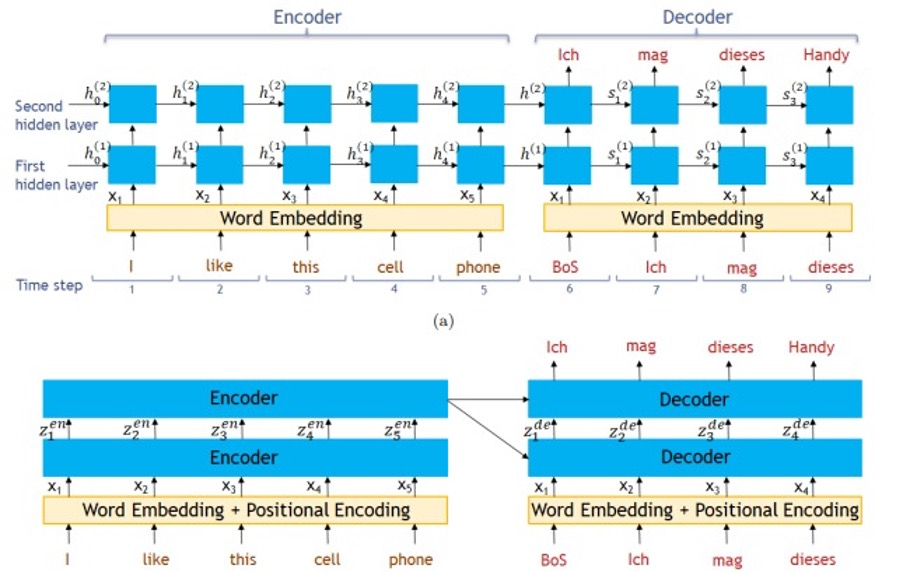
\includegraphics[width=1\textwidth]{Picture4.jpg}
\end{center}

An example of a simple language translation task performed using (a) a classical model, such as an RNN, LSTM, or GRU, and (b) a Transformer.

\subsubsection{Multi-Head Self-Attention}
The input data X may contain several levels of correlation information and the learning process may benefit from processing the input data in multiple different ways. Multiple self-attention heads are introduced that operate on the same input in parallel and use distinct weight matrices Wq, Wk, and Wv, to extract various levels of correlation between the input data. For example, consider the sentence “Do we have to turn left from here or have we left the street behind?”. There are two occurrences of the word “left” in the sentence. Each occurrence has a different meaning, and consequently a different relationship with the rest of the words in the sentence. Transformers can capture such information by using multiple heads. Each head is built using a separate set of query, key, and value weight matrices and computes self-attention over the input sequence in parallel with other heads. The use of multiple heads in a Transformer is analogous to using multiple kernels at each layer in
convolutional neural network, where each kernel is responsible for learning distinct features or representations.

Step 1: Generation of Multiple Sets of Distinct Query, Key, and Value Vectors
Step 2: Scaled Dot Product Operations in Parallel
This step consists of implementing the following relationship, as shown in the figure:

\begin{center}
    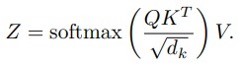
\includegraphics[width=.5\textwidth]{Picture6.jpg}
\end{center}

Step-3 - Concatenating and Linearly Combining Outputs
	It is important to note that the input and output of the multi-head self-attention are of the same dimension, that is, dimension (X) = dimension (Z).

\begin{center}
    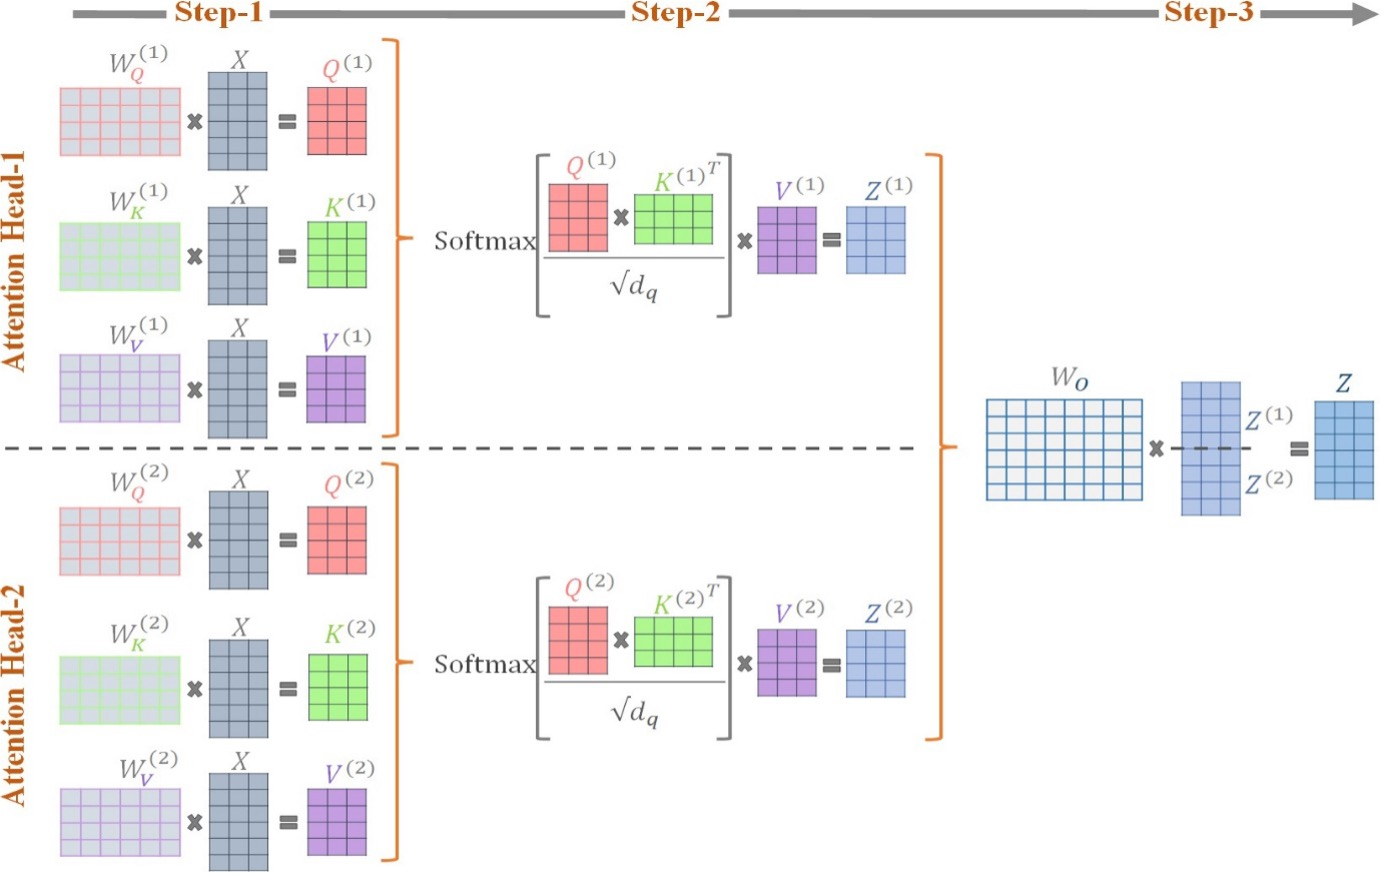
\includegraphics[width=1\textwidth]{Picture5.jpg}
\end{center}

\subsubsection{Positional Encoding}
Transformers successfully avoided the recurrence and unlocked a performance bottleneck of sequential operations.
But now there is a problem. By processing all the positions in a sequence in parallel, the model also loses the ability to 
understand the relevance of the position. For the Transformer, each position is independent of the other, and hence one key 
aspect we would seek from a model that processes sequences is missing. The original authors did propose a way to make sure we 
do not lose this information—positional encoding

\begin{center}
    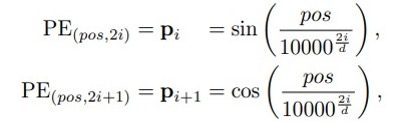
\includegraphics[width=.5\textwidth]{Picture7.jpg}
\end{center}

Where \textit{pos} is the position (time-step) in the sequence of input words. If the input, $\mathbf{X}$, is a $d_{\text{model}}$-dimensional embedding for $n$ tokens in a sequence, positional embedding, $\mathbf{P}$, is a matrix of the same size ($n \times d_{\text{model}}$). The element on the $\text{pos}^{th}$ row and $2i^{th}$ or $(2i + 1)^{th}$ column is defined as follows.

\begin{center}
    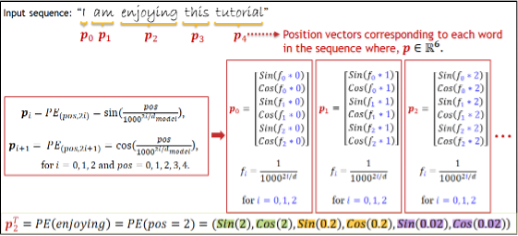
\includegraphics[width=1\textwidth]{Picture8.png}
\end{center}

\subsection{Summary}
In recent chapters, we covered fundamental concepts and building blocks of deep learning for time series forecasting, applying them practically using PyTorch. We intentionally postponed attention mechanisms and Transformers for a dedicated chapter. We introduced the generalized attention model, explored specific attention schemes, and seamlessly integrated attention into Seq2Seq models. Transitioning to the Transformer, we adapted its architecture for time-series applications, concluding with training a Transformer model for forecasting on a household sample. This chapter lays the groundwork for using deep learning in time series forecasting. The next chapter will explore the global forecasting model paradigm.

\section{Chapter 14 Code Analysis}

\subsection{Code}
\href{https://github.com/mijanr/TimeSeries/blob/master/Time_Series_Classification/cnn_plus_lstm.ipynb}{GitHub reference link}

\subsection{Conclusion}
Each strategy has advantages and disadvantages of its own, and the optimal option will rely on the particular issue at hand. All things considered, combining CNNs with LSTMs can offer a potent tool for handling a variety of sequence learning problems.

\subsection{Research Summary}

\subsection{Encoder-Decoder Transformer Architecture}
The encoder-decoder transformer architecture can be represented mathematically as follows \\
E = Encoder(X) \\ 
D = Decoder(E) \\
\subsubsection{Encoder Mechanism}
The encoder mechanism can \\
    Z = [Q(X), K(X), V(X)] \\
    H = [ Attention(Z), PositionalEncoding(X) ] \\
    E = Feedforward(H) \\ \\
where:
\begin{itemize}
    \item $Q$, $K$, and $V$ are matrices representing the query, key, and value vectors, respectively.
    \item  Attention is a function that computes the attention scores between the query vector and the key vectors.
    \item PositionalEncoding is a function that adds positional information to the input text.
    \item Feedforward is a neural network that performs a series of non-linear transformations.
\end{itemize}

\subsubsection{Decoder Mechanism}
The decoder mechanism can be represented mathematically as follows: \\
Y = [Q(Yt), K(Yt), V(Yt)] \\
M = [MaskedAttention(Z, Yt), DecoderSelfAttention(Yt)] \\
N = [EncoderDecoderAttention(Z, Yt)] \\
H = [M, N] \\
D = Feedforward(H) \\
Y = Yt + D \\ \\
where:
\begin{itemize}
    \item Yt is the output sequence of tokens at time step t.	
    \item MaskedAttention is a function that computes the masked attention scores between the query vector and the key vectors, where the attention is masked to prevent the decoder from attending to future tokens in the output sequence.
    \item DecoderSelfAttention is a function that computes the decoder self-attention scores between the query vector and the key vectors, which allows the decoder to attend to different parts of its output text.
    \item EncoderDecoderAttention is a function that computes the encoder-decoder attention scores between the query vector and the key vectors, which allows the decoder to attend to the input text.
    \item Feedforward is a neural network that performs a series of non-linear transformations.

\end{itemize}

\subsection{Attention Mechanism}
The attention mechanism can be represented mathematically as follows \\
\[S = Q * K^T ,  \\ 
A = Softmax(S) , \\
V = A * V \] \\ 
where:
\begin{itemize}
    \item Y is the set of all possible outputs.
    \item P(Y) is the probability distribution over the possible outputs.
    \item D is the output of the decoder.
\end{itemize}

\subsection{Probabilistic Forecasting}
Transformer models can be used to generate probabilistic forecasts by using a softmax function to output a probability distribution over the possible outputs. This can be written mathematically as follows \\
\[P(Y) = Softmax(D) \] 
where:
\begin{itemize}
    \item Y is the set of all possible outputs.
    \item P(Y) is the probability distribution over the possible outputs.
    \item D is the output of the decoder.
\end{itemize}

\subsection{Softmax function}
The softmax function is a function that is used to convert a vector of real numbers into a vector of probabilities. It is often used in neural networks to normalize the output of a layer before it is passed to the next layer.
The softmax function can be represented mathematically as follows \\

\[ S = Q \cdot K^T \] \\ 
where:
\begin{itemize}
    \item Z is the vector of real numbers.
    \item S is the vector of probabilities. 
\end{itemize}

The softmax function works by taking a vector of real numbers and calculating the exponential of each number. It then divides each number by the sum of the exponentials. This ensures that the sum of the probabilities is equal to 1.
The softmax function is a very important function in neural networks because it allows the network to learn complex relationships between the inputs and the outputs. It is also used to normalize the output of the network, which helps to prevent the network from overfitting to the training data.

Here is an example of how the softmax function can be used to normalize a vector of real numbers:
\[ Z = [1, 2, 3] \]
\[S = e^(Z)/Sum(e^(Z)) \]
\[S = [2.7183, 7.3891, 20.0855]/30.9505\]
\[S = [0.0930, 0.2397, 0.6673]\]
As you can see, the softmax function has normalized the vector of real numbers to a vector of probabilities. The sum of the probabilities is equal to 1.

\subsection{Positional encoding } 
\subsubsection{Positional Encoding with Sinusoids}
One common method for positional encoding involves using sinusoidal functions to represent the relative positions of tokens. This approach is widely used in the transformer architecture due to its effectiveness in capturing long-range dependencies between tokens.
The basic idea behind positional encoding with sinusoidal functions is to add a set of additional vectors to the input representation, where each vector represents a specific position in the sequence. These vectors are typically created using sine and cosine functions, which vary with the position index.
The specific implementation of positional encoding with sinusoidal functions involves multiplying the input representation by a matrix of positional encoding vectors. This matrix is constructed by generating a set of sine and cosine functions for each position in the sequence. The functions have different frequency and offset values for different positions, allowing the model to capture information about the relative distances between tokens.
The resulting positional encoding vector is then added to the input representation, effectively embedding the positional information into the model's internal representation of the input sequence.
The mathematical formulation for positional encoding with sinusoidal functions can be expressed as follows \cite{r5} \\
\[ PE(pos) = sin(pos / (10000^2)) + cos(pos / (10000^2)) \]
where:
\begin{itemize}
    \item PE(pos) is the positional encoding vector for position pos.
    \item 10000 is the embedding dimension.
\end{itemize}
This formulation generates positional encoding vectors with a period of 10,000, which is sufficient for capturing long-range dependencies in natural language sequences.

\subsubsection{Positional Encoding with Learned Parameters}
While using pre-trained positional encoding vectors is a common approach, there have been studies that explore the use of learned positional encoding parameters. This approach involves introducing additional parameters to the model that are specifically responsible for learning positional information. The parameters are typically learned during the training process, allowing the model to adapt the positional encoding to the specific characteristics of the training data.
The mathematical formulation for learned positional encoding can be expressed as follows \\
\[ PE(pos) = W_pos * pos + b_pos \]
where:
\begin{itemize}
    \item PE(pos) is the positional encoding vector for position pos.
    \item Wpos is the weight matrix for positional encoding.
    \item bpos is the bias vector for positional encoding.
\end{itemize}

This formulation allows the model to learn a more adaptive and task-specific representation of positional information.

\subsection{Token} 
The input sequence of tokens in the transformer model is generated by splitting the input text into individual words or subwords. This process is called tokenization. Tokenization is necessary because the transformer model cannot work with raw text. It needs to process the text as a sequence of tokens, which are then represented as vectors of numbers. \\ \\
Two main types of tokenization: 
\begin{itemize}
    \item byte pair encoding: BPE is a more sophisticated approach that can split words into smaller subwords, which can be helpful for languages with complex morphology.
    \item Wordpiece is a simpler approach that only splits words into subwords if necessary.
\end{itemize}
Once the input text is tokenized, the transformer model can then process it as a sequence of vectors. These vectors are then passed through the encoder and decoder layers, where they are transformed and combined to generate the output sequence of tokens.

\subsection{Data Flow}
The transformer model takes an input sequence of tokens and passes it through the encoder, which transforms it into a latent representation. The decoder then takes the latent representation and generates an output sequence of tokens. The decoder is able to generate the output sequence by attending to different parts of the input sequence and its own output sequence. \\

The data flow through the transformer model can be mathematically represented as follows: \\ 
\[ X = InputSequence \]
\[E = Encoder(X) \]
\[Z = LatentRepresentation(E) \]
\[Y = Decoder(Z) \]
\[OutputSequence = Y \]
The encoder transforms the input sequence into a latent representation using the encoder layers. The decoder generates the output sequence using the latent representation and the decoder layers.

\section{Chapter 15 Summary}

\subsection{Introduction}
The chapter discusses strategies for enhancing global deep learning forecasting models. It addresses the challenges in forecasting and introduces various features and techniques to improve model performance.

\subsection{Creating global deep learning forecasting models}
Chapter 10 emphasizes the importance of global forecasting models in the context of deep learning. Key points include:
\begin{itemize}
    \item Global models offer advantages like increased data size, cross-learning, multi-task learning, regularization, and reduced engineering complexity.
    \item Deep learning models require substantial data, making global models a compelling choice.
    \item Transitioning from individual to global models is facilitated by adapting the data loader to sample from multiple time series.
    \item The PyTorch Forecasting library simplifies time series forecasting with deep learning, offering a high-level API and a TimeSeriesDataset class for data preparation.
\end{itemize}

In summary, Chapter 10 highlights the benefits of global models in deep learning forecasting and introduces tools like PyTorch Forecasting to streamline model development. 
In the first implementation, there is only one decoder in each timestep and target sequence. The model is trained exclusively on the historical data, and its task is to predict future values based solely on this historical information. This approach simplifies the forecasting process, making predictions based on the past without considering complex multi-sequence interactions or external factors.


\subsection{Using time-varying information}
In this context, we face a challenge when setting up the model due to the nature of historical data. We need to consider that time-varying known features and the history of the target variable cannot be used together for single-step-ahead forecasting. This is because the time-varying features have future values known in advance, making them suitable for prediction at a given timestep. In contrast, the history of the target variable lacks this advantage, as it represents the quantity we aim to forecast, leading to a causal constraint. The current tensor arrangement aligns these two types of data on the same timesteps, which needs to be addressed to avoid inappropriate forecasting.



\subsection{Using static/meta information}

Incorporating household-specific features, like the Acorn group and dynamic pricing, into the model allows it to capture unique patterns associated with different households. Categorical features, which are non-numeric, can pose challenges in machine learning models. However, in deep learning models, there is a distinct approach for handling these categorical features called embedding vectors. This technique involves converting categorical variables into continuous vector representations, making them suitable for neural networks. This allows the model to learn complex relationships and patterns within categorical data, enhancing its forecasting capabilities.
\begin{itemize}
    \item \textbf{One-hot encoding: } Transforms categorical data into a high-dimensional binary format, with each category becoming a dimension. This method creates a sparse representation, adding dimensions equal to the category count. However, it treats all categories as equally distant, disregarding potential similarities. For instance, it fails to capture that Saturday and Sunday are closer as weekend days.
    \item \textbf{Embedding vectors: } offer a dense representation of categorical features through an embedding layer, which maps each category to a numerical vector. These vectors have lower dimensions than the categorical feature's cardinality. During training, the model determines the optimal vector for each category. This approach is common in natural language processing, where it's used to embed thousands of words into dimensions as small as 200 or 300.
\end{itemize}




\subsection{Using the scale of the time series}

To scale time series data, GroupNormalizer in TimeSeriesDataset is used to make the target zero mean and unit variance. This prevents the model from adjusting its parameters based on individual household consumption scales. However, it results in information loss because unique patterns in larger and smaller consumption households are combined. To reintroduce this scale information without including unscaled targets, mean and standard deviation data for each household, collected during the initial scaling process, can be added as static-real features to the model. This provides the model access to scale information while learning time series patterns.



\subsection{Balancing the sampling procedure}
The analogy of the bowl and chits of papers is used to explain the concept of balancing the sampling procedure in the context of selecting batches from time series data. Imagine the bowl filled with balls, where each ball represents a time series (household), and the chits of paper represent different windows of samples that can be drawn from each time series.

In the default batch sampling procedure, all the chits are dumped into the bowl, and a batch is randomly selected by picking a certain number of chits. This can result in a biased batch composition, especially if there is an imbalance in the characteristics of the time series, such as different lengths or consumption levels.

To address this bias, a threshold-based sampling approach is introduced. Instead of uniformly selecting chits, a random number between 0 and 1 (p) is generated for each chit, and the chit is selected only if p is less than a certain threshold (e.g., p < 0.5). By adjusting this threshold, it becomes possible to control the acceptance rate of chits, making it harder or easier for a chit to be included in the batch.

The goal is to find the right thresholds for each chit so that the resulting batch has a more balanced representation of different characteristics (represented by colors in the analogy). To achieve this, the thresholds are determined based on the inverse of the count of chits in each category or bin. Bins with fewer samples get higher weights, making it more likely for their chits to be selected, while bins with more samples have lower weights, reducing their chances of inclusion. This strategy helps create batches with a more even distribution of different characteristics.

\subsection{Summary}
In recent chapters, we've laid the groundwork for deep learning models and explored the concept of global models in deep learning. We've utilized PyTorch Forecasting and the versatile TimeSeriesDataset for model development.

Starting with a basic LSTM in the global context, we expanded our models by incorporating time-varying, static, and individual time series scale information, enhancing their performance. We also delved into an alternating sampling approach for mini-batches to ensure balanced representation in each batch.

While this chapter provides valuable techniques for improving forecasting models, it serves as a foundation for further model development. In the upcoming chapter, we'll explore specialized deep learning architectures tailored for time series forecasting.


\subsection{Using Static/Meta Information}
The chapter explores the inclusion of static/meta information, such as Acorn group, dynamic pricing, etc., in forecasting models. Categorical features are discussed, highlighting the challenges of using one-hot encoding due to its sparsity. The introduction of embedding vectors as a dense representation for categorical features in deep learning models is explained.

\subsection{Embedding Vectors and Dense Representations}
An embedding layer is introduced to handle categorical features, providing a mapping between each categorical value and a numerical vector. The embedding layer is trained along with the network, allowing the model to learn the best vector representation for each categorical value.

\subsection{Defining a Model with Categorical Features}
The \texttt{StaticDynamicFeatureRNNModel} is presented, incorporating static and time-varying categorical features. The initialization of the model includes embedding layers for categorical features, and thumb rules for choosing embedding sizes are discussed.

\subsection{Scale of the Time Series}
The chapter addresses the information loss in scaling time series and proposes adding scale information as static-real features to the model. The use of \texttt{add\_target\_scales} parameter in \texttt{TimeSeriesDataset} for scaling is introduced.

\subsection{Balancing the Sampling Procedure}
The sampling procedure for global modeling is discussed, emphasizing the importance of balanced sampling. The analogy of balls in a bowl is used to explain the sampling process. The chapter introduces weighted random sampling using \texttt{WeightedRandomSampler} to achieve a more balanced distribution in batches.

\subsection{Visualizing Data Distribution and Results}
The length distribution of time series is visualized using bins, and the impact of sampling strategies on batch distribution is shown through stacked bar charts. Results after training the model with the enhanced sampling technique are presented.

\subsection{Summary}
The chapter concludes by emphasizing the importance of experimentation and hypothesis testing in improving forecasting models. It provides insights into different strategies and encourages readers to explore further for optimal model performance.

\section{Wavelet Analysis}
\subsection{What is Wavelet Analysis} 
Wavelet analysis is a mathematical technique used for analyzing and representing signals, images, and other data in both time and frequency domains. It is particularly useful for capturing localized variations in a signal, making it well-suited for applications such as signal processing, image compression, and data compression.

The basic idea behind wavelet analysis is to decompose a signal into different frequency components at various scales. This is in contrast to traditional Fourier analysis, which represents a signal solely in terms of its frequency components. The wavelet transform uses a set of functions called wavelets, which are small, localized functions that are well-suited for capturing short-duration events or features in a signal.

\section{Wavelet Transforms}
Wavelet transforms are mathematical tools for analyzing data where features vary over different scales. For signals, features can be frequencies varying over time, transients, or slowly varying trends. For images, features include edges and textures. Wavelet transforms were primarily created to address the limitations of the Fourier transform.

While Fourier analysis consists of decomposing a signal into sine waves of specific frequencies, wavelet analysis is based on decomposing signals into shifted and scaled versions of a wavelet. A wavelet, unlike a sine wave, is a rapidly decaying, wave-like oscillation. 

\section{Wavelet Time Scattering} 
Wavelet time scattering is a signal processing technique that involves decomposing a signal into different time scales using wavelet transforms. It's often used for feature extraction in time-series analysis. In MATLAB, the Scattering Transform Toolbox (ScatNet) is a popular toolbox for wavelet time scattering.


\subsection{Wavelet Time Scattering for ECG Signal Classification} 
\subsubsection{Code Analysis} 
This example utilizes the Statistics and Machine Learning Toolbox along with the Wavelet Toolbox to demonstrate the classification of human electrocardiogram (ECG) signals. The approach involves wavelet time scattering and a support vector machine (SVM) classifier. Wavelet scattering involves a series of transformations, nonlinearities, and averaging to generate low-variance representations of time series, ensuring insensitivity to shifts in the input signal while maintaining class discriminability. The necessary toolboxes for running this example are the Wavelet Toolbox™ and the Statistics and Machine Learning Toolbox™. The publicly available ECG data used in this example is sourced from Physio Net. For alternative approaches, a deep learning method is explored in the example "Classify Time Series Using Wavelet Analysis and Deep Learning," and a machine learning approach is detailed in "Signal Classification Using Wavelet-Based Features and Support Vector Machines." In the context of wavelet scattering, the term "time windows" refers to the number of samples obtained after downsampling the output of the smoothing operation. 

\subsubsection{Data Description}
This example employs electrocardiogram (ECG) data obtained from three distinct groups: individuals with cardiac arrhythmia, individuals with congestive heart failure, and individuals with normal sinus rhythms. The dataset comprises 162 ECG recordings from three PhysioNet databases: MIT-BIH Arrhythmia Database, MIT-BIH Normal Sinus Rhythm Database, and The BIDMC Congestive Heart Failure Database. Specifically, there are 96 recordings from individuals with arrhythmia, 30 recordings from individuals with congestive heart failure, and 36 recordings from individuals with normal sinus rhythms. The primary objective is to train a classifier capable of distinguishing between arrhythmia (ARR), congestive heart failure (CHF), and normal sinus rhythm (NSR).

For data acquisition, the first step involves downloading the data from the GitHub repository. This includes the physionet$_ECG_data-main.zip file, which, when extracted, contains ECGData.zip and README.md$

\subsubsection{Loading data}
This section outlines the process of loading files and preparing the dataset for classification. I have downloaded ECG classification data from GitHub provided by Matlab.

\subsubsection{Creating Training and Validation datasets }
To create training and test datasets, the data is randomly split using the helper function helperRandomSplit. In this instance, 70 percent of the data is designated for the training set, and the remaining 30 percent is allocated to the test set. The resulting datasets, namely trainData, testData, trainLabels, and testLabels, are organized for subsequent classification tasks.

Dataset statistics reveal that the training set comprises 113 records, while the test set contains 49 records. The distribution of each class in the training and test sets is examined, demonstrating consistency with the overall class percentages in the original dataset (ARR: 59.26%, CHF: 18.52%, NSR: 22.22%).

\subsubsection{Plot Sample}

This section involves visualizing the ECG waveforms by plotting the first few thousand samples of four randomly selected records from the ECGData. The provided helper function, helperPlotRandomRecords, facilitates this task. The function takes ECGData and a random seed as inputs. The initial seed is set to 14 to ensure that at least one record from each class is plotted.

\begin{figure}
  \centering
  \includegraphics[width=0.5\textwidth]{Images/plott.png} % Replace 'example-image' with the actual filename of your image
  \caption{Plot}
  \label{fig:sample}
\end{figure}


\subsubsection{Wavelet Time Scattering}
The key parameters to specify in a wavelet time scattering network are the scale of the time-invariant, the number of wavelet transforms, and the number of wavelets per octave in each of the wavelet filter banks. In many applications, the cascade of two filter banks is sufficient to achieve good performance. In this example, I construct a wavelet time scattering network with the default filter banks: 8 wavelets per octave in the first filter bank and 1 wavelet per octave in the second filter bank. The invariance scale is set to 150 seconds.
For classification, two analyses are performed. The first uses all the scattering data and fits a multi-class SVM with a quadratic kernel. In total, there are 2592 scattering sequences in the entire dataset, 16 for each of the 162 signals. The error rate, or loss, is estimated using 5-fold cross-validation.

\begin{figure}
    \centering
    \includegraphics[width=0.5\textwidth]{Images/image2.png}
    \caption{Filters}
    \label{fig:enter-label}
\end{figure}

\subsubsection{SVM Classification}
For the next analysis, I fit a multi-class quadratic SVM to the training data only (70 percent ) and then use that model to make predictions on the 30 percent of the data held out for testing. There are 49 data records in the test set. Use a majority vote on the individual scattering windows.

\begin{figure}
    \centering
    \includegraphics[width=0.5\textwidth]{Images/CF.png}
    \caption{Confusion Matrix}
    \label{fig:enter-labe}
\end{figure}

\subsubsection{Dependencies}
Given code in example had some matlab dependencies.to over come the errors during running this code i had to install some toolboxes such as machine learning tool box ,wavelet tool box ,signal processing toolbox,digital signsl toolbox.

\subsubsection{Summary}
In this study, I  employed wavelet time scattering and a support vector machine (SVM) classifier to categorize ECG waveforms into three diagnostic classes. The wavelet scattering technique emerged as a potent feature extractor, requiring minimal user-specified parameters while delivering robust features for classification. This stands in contrast to another approach, as demonstrated in the example "Signal Classification Using Wavelet-Based Features and Support Vector Machines," which demanded considerable expertise for manual feature crafting.

With wavelet time scattering, users only needed to specify the scale of time invariance, the number of filter banks (or wavelet transforms), and the number of wavelets per octave. The combination of wavelet scattering and SVM classification yielded impressive results. The cross-validated model achieved a remarkable 100 percent classification accuracy, highlighting the method's robustness. Additionally, when applying the SVM to the scattering transforms of a hold-out test set, a high accuracy of 98 percent  was attained. This underscores the efficacy of wavelet time scattering as a powerful and user-friendly tool for ECG waveform classification, offering a streamlined alternative to traditional manual feature engineering approaches.


\section{Chapter 16 Summary}

\subsection{The need for specialized architectures}

\begin{enumerate}
    \item \textbf{Inductive Bias in Deep Learning:}
    \begin{itemize}
        \item Refers to assumptions a learning algorithm makes to generalize from training to unseen data.
        \item Despite the belief that deep learning is purely data-driven, inductive biases are embedded within the architecture design.
    \end{itemize}
    
    \item \textbf{Impact of Inductive Bias:}
    \begin{itemize}
        \item Specific biases make certain architectures better for particular types of data.
        \item CNNs are optimized for image data due to spatial biases.
        \item RNNs were favored for sequential data due to their auto-regressive biases.
    \end{itemize}
    
    \item \textbf{Evolution of Models:}
    \begin{itemize}
        \item Transformers introduced with weaker sequence biases, leading to improved performance with adequate data.
    \end{itemize}
    
    \item \textbf{Designing DL Architectures:}
    \begin{itemize}
        \item The selection of inductive biases is critical when designing deep learning architectures.
        \item It's especially important for time series forecasting where model choice significantly affects outcomes.
    \end{itemize}
    
    \item \textbf{Specialized Architectures for Time Series:}
    \begin{itemize}
        \item The impracticality of training individual models for each time series in large-scale data necessitates specialized architectures.
        \item Focus on architectures that can handle the global modeling paradigm to accommodate forecasting at scale.
        \item \textbf{Neural Basis Expansion Analysis for Interpretable Time Series Forecasting (N-BEATS):}
        \begin{itemize}
            \item Introduced as a significant model for time series forecasting.
            \item Supported by stable open-source frameworks, making it accessible for practical application.
        \end{itemize}
    \end{itemize}
    
    \item \textbf{Scope of Discussion:}
    \begin{itemize}
        \item Not all architectures will be covered, but those that have made a lasting impact on the field will be.
        \item The chapter will guide the reader to additional resources for further exploration of time series forecasting models.
    \end{itemize}
\end{enumerate}

\subsection{Hybrid Foundations and Innovation in Time Series Forecasting: The N-BEATS Model}

\textbf{N-BEATS Overview:} \\
N-BEATS is a mix of deep learning (DL) and traditional statistical forecasting methods. It gained attention by winning the M4 forecasting competition in 2018.

\textbf{Origin of N-BEATS:} \\
\begin{itemize}
  \item Created by Slawek Smyl from Uber, it combined exponential smoothing with an RNN, resulting in the ES-RNN model.
\end{itemize}

\textbf{Significance in Forecasting:} \\
\begin{itemize}
  \item It sparked a discussion, led by Makridakis and others, about the effectiveness of combining different forecasting methods.
\end{itemize}

\textbf{Design Philosophy:} \\
\begin{itemize}
  \item N-BEATS was developed to prove that a purely deep learning-based model could excel in time series forecasting.
\end{itemize}

\textbf{Achievement:} \\
\begin{itemize}
  \item The model outperformed all others in the M4 competition, although it was not officially entered.
\end{itemize}

\textbf{Architecture:} \\
\begin{itemize}
  \item N-BEATS's design is heavily influenced by signal processing techniques.
\end{itemize}

\textbf{Forecasting Approach:} \\
\begin{itemize}
  \item Focuses on univariate forecasting, which relies only on past data to predict future data points.
  \item Does not use additional variables (covariates) for predictions.
\end{itemize}

\textbf{Model Input and Output:} \\
\begin{itemize}
  \item The model looks at a historical window of data (lookback period) to predict upcoming time steps (forecast period).
\end{itemize}

\subsection{Understanding N-BEATS: An Innovative Architecture for Time Series Forecasting}

\begin{figure}
    \centering
    \includegraphics[width=0.5\textwidth]{Images/Picture9.png}
    \caption{Confusion Matrix}
    \label{fig:enter-labe}
\end{figure}

\textbf{Block Structure:} \\
The basic building unit of the N-BEATS architecture is a "block". Each block receives an input based on the lookback period of a time series and produces two outputs: a forecast for the future and a backcast for the input period.

\textbf{Fully Connected (FC) Layers:} \\
Each block contains a stack of fully connected layers that transform the input into a hidden representation. This hidden representation is then processed to create expansion coefficients for both the forecast and backcast.

\textbf{Basis Layers:} \\
Expansion coefficients are passed through basis layers to generate the final forecast and backcast outputs. These basis layers can be designed to make the model's outputs interpretable, such as capturing trends or seasonality in the time series.

\textbf{Stacks of Blocks:} \\
Blocks are organized into "stacks". Each stack contains several blocks with shared characteristics, like the type of basis function they use. Stacks are arranged in a residual learning framework, where the backcast from one block is subtracted from its input to refine the signal for the next block.

\textbf{Global Forecasting:} \\
Stacks are chained together to form the overall N-BEATS model. The output of each stack is a forecast and a residual, with the residuals being passed as inputs to subsequent stacks. The final forecast of the model is an aggregate of all the forecasts from the individual stacks.

\textbf{Generic and Interpretable Modes:} \\
N-BEATS can operate in two modes—generic and interpretable. The generic mode does not impose any specific structure on the basis functions, while the interpretable mode uses predefined basis functions that enhance human understanding of the model's outputs.

\textbf{Implementation and Training:} \\
The architecture is implemented in PyTorch Forecasting, allowing for customization of stack types, the number of blocks, layer configurations, and expansion coefficients. This flexibility enables the model to forecast at different time horizons and provides a means to understand and interpret the model's internal representations.

\textbf{Competitive Performance:} \\
N-BEATS has been shown to perform competitively in time series forecasting challenges, highlighting the effectiveness of deep learning architectures that are designed with careful consideration of inductive biases and interpretability.

\subsection{Enhanced Forecasting with N-BEATS: Interpretable Outputs and Integration of Exogenous Variables}

\begin{figure}
    \centering
    \includegraphics[width=0.5\textwidth]{Images/Picture10.png}
    \caption{Confusion Matrix}
    \label{fig:enter-labe}
\end{figure}


\textbf{N-BEATS Model Overview:} \\
It offers an interpretable mode, separating forecasts into components like trend and seasonality. To obtain this detailed output, modify the predict function parameter from mode="prediction" to mode="raw".

\textbf{Interpretable Outputs:} \\
The model returns a namedtuple with separate keys for trend (trend), seasonality (seasonality), and the overall prediction (prediction).

\textbf{Example of Decomposed Forecast:} \\
The figure titled "Decomposed predictions from N-BEATS (interpretable)" showcases an example of a decomposed forecast. It visualizes actual data points (Target) against the model's predictions, with clear delineations of trend and seasonality components.

\textbf{Univariate Model Limitations:} \\
Initially, N-BEATS was designed as a univariate model, using only historical data for predictions, without external influences. This was sufficient for the M4 competition, which focused on univariate time series.

\textbf{Incorporating Exogenous Variables:} \\
To handle real-world datasets that include additional, explanatory (exogenous) variables, modifications were made to the original N-BEATS model. These modifications allow the inclusion of external information in the forecasting process, enhancing the model's applicability to more complex scenarios.

\subsection{Enhancing Time Series Forecasting with N-BEATSx: Integrating Exogenous Variables}

\begin{figure}
    \centering
    \includegraphics[width=0.5\textwidth]{Images/Picture11.png}
    \caption{Confusion Matrix}
    \label{fig:enter-labe}
\end{figure}


\textbf{N-BEATSx Model Extension:} \\
The image discusses an enhancement to the N-BEATS model, known as N-BEATSx, allowing it to incorporate additional variables into forecasting.

\textbf{Incorporation of Exogenous Variables:} \\
Unlike N-BEATS, which only uses past data (univariate), N-BEATSx can use external or exogenous variables in its predictions.

\textbf{Forecasting with Exogenous Variables:} \\
The formula in the image shows how N-BEATSx creates a forecast using a linear combination of exogenous variables. It assigns weights to these variables using expansion coefficients, which are learned during the model training process.

\textbf{Interpretable and Generic Blocks:} \\
N-BEATSx introduces two types of blocks for handling exogenous data:

\begin{itemize}
  \item \textbf{Interpretable Exogenous Blocks:} These allow for understanding the contribution of each exogenous variable to the forecast.
  \item \textbf{Generic Exogenous Blocks:} These process exogenous variables through an encoder but do not provide the same level of interpretability.
\end{itemize}

\textbf{Context Vector Learning:} \\
For the generic version, a context vector is learned for the exogenous variables, which then contributes to the forecast.

\textbf{Temporal Encoders:} \\
Two types of encoders, TCN and WaveNet, are suggested for learning from time-varying exogenous data.

\textbf{Implementation and Limitations:} \\
N-BEATSx is not available in PyTorch Forecasting but can be found in the neuralforecast library, which has its own set of limitations, such as not supporting categorical features natively.

\textbf{Performance:} \\
The N-BEATSx model has demonstrated superior performance over N-BEATS and other benchmarks in tasks like electricity price forecasting.

\textbf{Model Suitability:} \\
The text hints at a further modification for long-term forecasting, suggesting ongoing enhancements to the N-BEATSx model.

\subsection{Max Pooling in N-HiTS: Enhancing Long-Horizon Forecasting Efficiency}

\begin{figure}
    \centering
    \includegraphics[width=0.5\textwidth]{Images/Picture13.png}
    \caption{Confusion Matrix}
    \label{fig:enter-labe}
\end{figure}

Illustration of Max Pooling: The image demonstrates the max pooling operation on a time series dataset, which is a critical step in the N-HiTS architecture designed for long-term forecasting.

Reduction Technique: Max pooling, with a kernel size of 2 and a stride of 2, reduces the complexity of the input time series by downsampling it, which is essential for managing the computational load in long-horizon forecasting.

Extraction of Salient Features: By selecting the maximum value within each window defined by the kernel size, max pooling ensures that the most prominent features of the data are retained.

Implementation in N-HiTS: The pooling operation is part of the multi-rate data sampling technique employed by N-HiTS, which allows the model to capture patterns at varying resolutions and frequencies within the time series data.

Enabling Hierarchical Interpolation: Following the max pooling, N-HiTS utilizes a hierarchical interpolation process, where the downsampled data is interpolated to forecast future values at the original data resolution.

Optimization for Long-horizon Forecasting: Such an approach significantly reduces memory usage and computational requirements, making N-HiTS an efficient architecture for forecasting over extended periods.

Visualization of the Pooling Process: The image serves as a visual aid, showing how the max pooling operation selects the highest values from the input time series, simplifying the data while preserving its most critical points.

Contribution to Hierarchical Architecture: The max pooling process depicted is integral to the hierarchical nature of N-HiTS, which systematically breaks down the forecasting problem into more manageable sub-tasks.

\subsection{Implementing N-HiTS for Time Series Forecasting}

N-HiTS Implementation: Uses PyTorch Forecasting, building on strategies from Chapter 15.
Exogenous Variables Support: Similar to N-BEATSx, but without a dedicated exogenous block.

Initialization Parameters:
\begin{itemize}
  \item \texttt{n\_blocks}: Number of blocks per stack (e.g., [1,1,1] for three stacks with one block each).
  \item \texttt{n\_layers}: Number or layers of FC (Fully Connected) with ReLU activation in each block (recommended value is 2).
  \item \texttt{hidden\_size}: Determines the number of units in FC layers per block.
  \item \texttt{static\_hidden\_size}: Size for encoding static features via an FC encoder, as discussed in N-BEATSx.
  \item \texttt{shared\_weights}: Indicates if weights for expansion coefficients are shared within stacks. Sharing is suggested in interpretable stacks.
  \item \texttt{pooling\_sizes}: Defines pooling size for each stack, with descending order recommended.
  \item \texttt{pooling\_mode}: Type of pooling operation, either 'max' or 'average'.
  \item \texttt{downsample\_frequencies}: List of integers for expressiveness ratios in each stack, affecting interpolation.
\end{itemize}

Code Availability: Full training code is in "02-N-HiTS.ipynb" notebook, Chapter 16. Two notebook variables control the training scope and model training.

Model Training Time: Training on full data is time-intensive.

Informer Model: A modified Transformer model for efficient long-term forecasting, dealing with expressiveness and computational challenges.
Transformer Challenges: Traditional models face issues with long sequences due to quadratic computational complexity.

Community Solutions: Research focuses on efficient Transformers using various optimization techniques.

Further Reading: The paper by Zhou et al. on the Informer model, and resources on efficient Transformers.

\subsection{Advanced Forecasting with the Informer Model: Integrating ProbSparse Attention and Generative Decoding}

\begin{figure}
    \centering
    \includegraphics[width=0.5\textwidth]{Images/Picture15.png}
    \caption{Confusion Matrix}
    \label{fig:enter-labe}
\end{figure}

Architecture Overview:

The Informer model adapts the Transformer architecture to enhance time series forecasting.
It integrates a uniform input representation to process both historical and contextual information.

Components of the Informer Model:

Encoder: Utilizes multi-head ProbSparse self-attention to process input data efficiently.
Decoder: Employs a generative-style decoder for long-term forecasting.

Uniform Input Representation:

Combines history embeddings with global timestamp information for a comprehensive input representation.
Uses convolutional layers for value embedding and learnable embeddings for capturing temporal information.

ProbSparse Attention:

An efficient attention mechanism that relies on probabilistic sparsity to focus on key query-key pairs.
Reduces computational complexity by sampling a subset of query-key pairs, maintaining attention quality.

Attention Distillation:

Implements distillation to prioritize dominant features in attention maps across layers.
Uses dilated convolutions for feature refinement, improving attention focus and reducing redundancy.

Generative-Style Decoder:

Generates the entire forecast horizon in a single forward pass, speeding up the prediction process.
Samples from the input sequence serve as the starting point for the decoder, streamlining the inferencing.

Implementation Aspects:

The original Informer model does not natively support exogenous variables but can be adapted to include them.
Customizable parameters such as the number of layers, attention heads, and sparsity factor allow for tailored model configuration.

\subsection{Decomposition and Auto-Correlation in Autoformer Architecture for Enhanced Time Series Forecasting}

Autoformer Model Overview:

Autoformer is an extension of the Informer model, with a focus on long-term forecasting.
It utilizes Uniform Input Representation and a generative-style decoder from the Informer model.

Key Features of Autoformer:

Auto-Correlation Mechanism: Replaces standard attention with a mechanism that identifies sub-series similarities based on periodicity, optimizing the model for capturing seasonality.
Time Series Decomposition: The model decomposes the input signal into trend-cyclical and seasonal components, focusing on the challenging task of capturing seasonality.

Encoder and Decoder Architecture:

\begin{itemize}
  \item \texttt{Encoder}: Utilizes the Auto-Correlation block for self-attention, adding each block's output back as a residual connection and decomposing the signal to focus on seasonality.
  \item \texttt{Decoder}: Samples from the end of the seasonal component, extending the input tensor to include both the sampled window and the prediction horizon, maintaining the autoregressive nature of the prediction.
\end{itemize}

Decomposition and Aggregation:

Employs Series Decomp blocks to separate and discard the trend, allowing the network to concentrate on seasonality.
Uses an aggregation mechanism that applies weights to sub-series rather than individual points, creating a weighted mixture of the seasonality patterns.

Implementation Considerations:

The architecture is designed to handle the stable trend-cyclical part of the time series separately from the seasonality, improving the model's focus and efficiency.
Provides an innovative approach to capturing time series seasonality, leveraging autocorrelation for sub-series similarity and aggregation.

Practical Application:

Suitable for datasets with strong seasonal patterns, like the London Smart Meter Dataset, demonstrating the capacity to learn and predict complex seasonal behaviors.

\begin{figure}
    \centering
    \includegraphics[width=0.5\textwidth]{Images/Picture16.png}
    \caption{Confusion Matrix}
    \label{fig:enter-labe}
\end{figure}

\textbf{Encoder Process:}

\begin{itemize}
  \item \textbf{Input}: The encoder receives the time series data that is to be predicted.
  \item \textbf{Auto-Correlation Self-Attention}: The model applies its auto-correlation mechanism to capture dependencies based on periodicity in the data.
  \item \textbf{Series Decomp (Decomposition)}: After auto-correlation, the series decomposition block separates the signal into seasonal and trend-cyclical components.
  \item \textbf{Feed Forward}: A neural network that processes the data further.
  \item \textbf{Residual Connection}: The output of the feed forward is combined with the input of the block to retain essential information and enhance learning.
\end{itemize}

This encoder process is repeated 'N' times as depicted by the label "Nx", each iteration possibly refining the model's understanding of the data.

\textbf{Decoder Process:}

\begin{itemize}
  \item \textbf{Seasonal Init (Initialization)}: The decoder begins with the seasonal component, setting the trend-cyclical part to zero to focus on learning the seasonality in the data.
  \item \textbf{Trend-Cyclical Init}: This part of the decoder considers the trend-cyclical component, initialized with the mean of the input data to establish a baseline trend.
  \item \textbf{Cross Attention}: The model applies auto-correlation between the encoder's output and the decoder's initialized components to align and learn from the series patterns.
  \item \textbf{Final Output}: The process culminates in a seasonal prediction, integrating the learned seasonal patterns with the trend information.
\end{itemize}

The figure's rightmost part shows the time series broken down into its components:

\begin{itemize}
  \item \textbf{Top graph}: The original time series data with all its variations.
  \item \textbf{Middle graph}: The seasonal part extracted from the data, emphasizing regular patterns repeating over time.
  \item \textbf{Bottom graph}: The trend-cyclical part representing the underlying trend and cyclic movements, isolated from seasonal fluctuations.
\end{itemize}

The architecture employs a layered approach, with multiple blocks in both the encoder and decoder ("Mx" for the decoder), suggesting a deep learning structure that refines the model's predictions through each layer.

The Autoformer's architecture aims to capture complex temporal dynamics, particularly focusing on seasonality, by decomposing the time series, learning patterns at different scales, and efficiently forecasting over long horizons.

\section{Chapter 17: Multi-Step Forecasting}

\subsection{Why multi-step forecasting?}
Most real-world applications of time series forecasting demand multi-
step forecasting, whether it is the energy consumption of a household or the sales of a product. This
is because forecasts are never created to know what will happen in the future, but to take some action
using the visibility we get.

Despite a more prevalent use case, multi-step forecasting has not received the attention it deserves.
One of the reasons for that is the existance of easy to implement classical statistical models or econometrics models 
such as \textit{ARIMA} and \textit{exponential smoothing} which include the multi-step strategy bundled within what we call a model. 

Another reason for the low popularity of multi-step forecasting is that is simply harder to implement. The more steps we extrapolate into the 
future, the more uncertainty in the predictions.

\subsection{Recursive strategy}
The oldest strategy, most intuitive, and most popular technique to generate multi-step forecast. 
After training a model for one-step-ahead predictions, we employ it recursively to produce forecasts for $H$ future timesteps. 
Initially, the model uses the window $\mathcal{W}(Y_T)$, which incorporates the most recent timestamp from the training data, 
to forecast the immediate next value, $\hat{y}_{T+1}$. This forecast, $\hat{y}_{T+1}$, is then integrated into the historical data, 
leading to a new window $\mathcal{W}(Y_T; \hat{y}_{T+1})$ that includes this forecast. 
The updated window serves as input for the model to predict the subsequent value, $\hat{y}_{T+2}$. 
This iterative process continues, extending the forecast horizon until we have obtained predictions for all $H$ timesteps.
This is the strategy that classical models like \textit{ARIMA} and \textit{exponential smoothing} use internally. 


\subsection{Direct strategy}
Under the direct strategy, we train $H$ distinct models, each designed to forecast a specific future timestep. 
These models utilize the same input window $\mathcal{W}(Y_t)$ but are independently trained to predict outcomes 
at different points within the forecast horizon. Consequently, this approach enables us to learn a unique set of 
parameters for each timestep, allowing the ensemble of models to establish a direct and independent mapping from the 
input window to each point in the forecast horizon $H$. This method has gained popularity alongside the rise of 
machine learning (ML)-based forecasting techniques. Practical implementations of this strategy within the ML context can be 
categorized into two methods: 

\begin{itemize}
    \item \textbf{Shifting Targets:} Involves training each model to forecast a future step by shifting the target output by the corresponding horizon length
    \item \textbf{Eliminating Features:} Involves training models by selectively using input features that are valid according to the forecasting rules, such as excluding certain lagged features that would not be available at the time of prediction.
\end{itemize}

\textbf{NOTE:} The two ways mentioned in the preceding list work nicely if we only have lags as features. For
instance, for eliminating features, we can just drop the offending lags and train the model.
But in cases where we are using rolling features and other more sophisticated features, simple
dropping doesn’t work because lag 1 is already used in calculating the rolling features. This
leads to data leakage.

\subsection{Joint strategy}
In the realm of multi-step time series forecasting, traditional models typically generate a single output, adhering to a Multiple Input, Single Output (MISO) framework. However, advancements in Deep Learning (DL) allow the configuration of models to produce multiple outputs simultaneously, leading to the development of the Joint Strategy or Multiple Input, Multiple Output (MIMO). This approach trains a singular model to predict the entire forecast horizon in one operation. 

\textbf{Training Regime:} The Joint Strategy involves the training of a multi-output model to forecast all timesteps within the horizon concurrently. Utilizing a window function, $\mathcal{W}(Y_t)$, the model is trained to predict a sequence of future values, $\hat{y}_{t+1}, \ldots, \hat{y}_{t+H}$, based on inputs drawn from the historical data. A loss function evaluates the model's predictions against actual future values, optimizing the model's parameters for accurate horizon-wide forecasting.

\textbf{Forecasting Regime:} Once trained, the model applies the same window function to new or unseen data, $\mathcal{W}(Y_T)$, to forecast the entire horizon in a single step. This capability is particularly leveraged in DL models by designing the last layer to output $H$ scalars, representing the forecast for each future timestep, rather than a single output.

This strategy's utilization predominantly in DL models showcases its compatibility with the architectural flexibility of neural networks, enabling the simultaneous prediction of multiple future values, enhancing forecasting efficiency and coherence across the forecast horizon.


\subsection{Hybrid strategies}
Over the year there has been efforts to implement hybrid strategies which combine the advatanges
of each of the strategies previously mentioned. Some of them are: \textit{DirRec Strategy}, \textit{Iterative block-wise strategy},
\textit{Rectify Strategy}, and \textit{RecJoint}. That being said, it is possible for each
user to come up with their own strategy.

\subsubsection{DirRec Strategy}
As the name suggest, it is a combination of direct and recursive strategies.
\begin{itemize}
    \item \textbf{Trainig Regime:} The DirRec strategy, standing for Direct-Recursive, innovatively blends aspects of both direct and recursive forecasting methodologies for multi-step forecasting over a horizon of \(H\). Unlike conventional approaches that either forecast each step independently (Direct) or recursively use each forecast as input for the next (Recursive), DirRec employs \(H\) distinct models. Each model is tailored to forecast a specific future step, starting with \(\mathcal{W}(Y_t)\) for the immediate next step. As a novel twist, models for steps beyond the first not only utilize the initial input window but also incorporate forecasts from all previous steps. Formally, for any given step \(h < H\), the model inputs include \(\mathcal{W}(Y_t)\) alongside all intermediary forecasts up to \(h\), thereby enriching the predictive context. This methodical incorporation of preceding forecasts into each subsequent model's training regime aims to capture a more comprehensive temporal pattern, potentially enhancing the accuracy and robustness of the overall forecasting strategy.
    \item \textbf{Forecasting Regime:} Similar to Training regime, but instead of training the models, we use the \(H\) trained models to generate the forecast in a recursive manner.
\end{itemize}

\subsubsection{Iterative block-wise strategy}
Also called the \textbf{iterative multi-SVR strategy}, tries to tackle the shortcomings of the 
direct strategy, which requires \(H\) different models to train, making it difficult for long scale-horizon forecasting. 
This is achieved by using a block-wise iterative style of forecasting.
\begin{itemize}
    \item \textbf{Trainig Regime:} Forecast horizon \(H\) is split into \(R\) blocks of lenght \(L\) such that \(H = L \times R\). And instead of training \(H\) direct models, we train \(L\) direct models.
    \item \textbf{Forecasting Regime:} We use the \(L\) trained models to generate a forecasts for the initial \(L\) timesteps (\(T + 1\) to \(T + L\)) within the forecast horizon \(H\), employing the window \(\mathcal{W}(Y_T)\). The first series of forecasts, denoted \(Y_{T+L}\), combined with the dataset \(Y_T\), is used to form a new window, \(\mathcal{W}(Y_T; Y_{T+L})\). This newly formed window then serves to predict the next \(L\) timesteps (\(T + L\) to \(T + 2L\)). This iterative approach is continued to cover the complete forecast horizon.
\end{itemize}

\subsubsection{Rectify Strategy}
It's another way to combine direct and recursive strategies by forming a two stage training and inferencing methodology. It can be seen 
as a model stacking approach but between different multi-step forecasting strategies.
\begin{itemize}
    \item \textbf{Trainig Regime:} It is done in two steps. Initially, a recursive approach forecasts the entire horizon \(H\), producing a preliminary set of predictions, \(\tilde{Y}_{t+H}\). Following this, for each horizon, direct models are trained, harnessing both the authentic historical data \(Y_t\) and the recursively derived forecasts \(\tilde{Y}_{t+H}\) as inputs.
    \item \textbf{Forecasting Regime:} Similar to the training, recursive forecasts are generated first and are used to generate the final forecast along the original history.
\end{itemize}

\subsubsection{RecJoint}
Is a mashup between the recursive and joint strategies, but applicable for single output models.
\begin{itemize}
    \item \textbf{Trainig Regime:} It trains a single model to recursively predict future values, utilizing the forecast at time \(t + 1\) as input for the subsequent prediction at \(t + 2\), and so on. \textit{RecJoint} generates forecasts for the entire horizon \(H\), conducting a joint optimization of these forecasts during training. This forces the model to concurrently consider all \(H\) timesteps, thereby achieveing a comprehensive horizon-wide optimization. Notably implemented in Seq2Seq models with RNN encoders and decoders.
    \item \textbf{Forecasting Regime:} It is the same as for the recursive strategy. 
\end{itemize}

\subsection{How to choose a multi-step forecasting strategy}
When choosing a which strategy to use it is important to take into consideration multiple perspectives, such as:
\begin{itemize}
    \item \textbf{Engineering complexity:} Recursive, Joint, RecJoint \(<<\) IBD \(<<\) Direct, DirRec \(<<\) Rectify
    \item \textbf{Training time:} Recursive \(<<\) Joint (typically \(T_{mo} > T_{so}\)) \(<<\) RecJoint \(<<\) IBD \(<<\) Direct, DirRec \(<<\) Rectify
    \item \textbf{Inference time:} Joint \(<<\) Direct, Recursive, DirRec, IBD, RecJoint \(<<\) Rectify
\end{itemize}

It also helps us to decide the kind of model we can use for each strategy. For instance, a joint strategy
can only be implemented with a model that supports multi-output, such as a DL model.

Some othe important guidelines to take into consideration when choosing the best multi-step forecasting strategy for each use case are the following:
\begin{itemize}
    \item In the recursive forecasting strategy, error components such as bias and variance at step \(h = 1\) directly influence the error at step \(h = 2\), leading to an accumulation of errors as the forecast horizon extends. This phenomenon results in increasing error variance over time, a characteristic that was empirically confirmed through studies showing significant variance escalation in recursive forecasts. In contrast, the direct strategy lacks this step-wise error dependence, thereby avoiding the recursive approach's error accumulation and ensuring more consistent forecast quality over the horizon.
    \item The direct forecasting strategy ensures that error components like bias and variance at step \(h = 1\) do not influence subsequent steps, as each \(h\) is forecasted independently. While this method avoids cumulative error, it may yield forecasts that lack coherence across the horizon, failing to account for potential dependencies between consecutive forecasts. This independence might lead to unrealistic predictions, particularly in time series characterized by non-linear trends, potentially resulting in a discontinuous forecast curve.
    \item Practically, in most cases, a direct strategy produces coherent forecasts.
    \item In recursive forecasting, models that generate highly variable forecasts can lead to an increased bias. This effect is particularly noticeable in complex models, which, despite their inherent low bias, introduce significant variability into forecasts. Such variability amplifies the bias within the recursive strategy, underscoring the nuanced relationship between model complexity, forecast variation, and bias amplification.
    \item In the context of large datasets, the bias term for the direct forecasting strategy approaches zero, contrasting with the recursive strategy, where bias remains nonzero. Empirical studies have shown that the direct strategy consistently outperforms the recursive strategy in scenarios involving long time series. This phenomenon is explained through learning theory, which posits that the direct strategy requires learning \(H\) distinct functions using the same dataset—a more complex task than learning a single function as in the recursive strategy. This difficulty is especially magnified in situations of data scarcity.
    \item Although the recursive strategy seems inferior to the direct strategy theoretically and empirically, it is not without some advantages:
    \begin{itemize}
        \item For highly non-linear and noisy time series, learning direct functions for all the horizons can be hard. And in such situations, recursive can work better.
        \item If the underlying \textbf{data-generating process (DGP)} is very smooth and can be easily approximated, the recursive strategy can work better.
        \item When the time series is shorter, the recursive strategy can work better.
    \end{itemize}
    \item The joint strategy mitigates the challenge of generating potentially unrelated forecasts across the forecast horizon—an issue inherent to the direct strategy. By evolving from the direct strategy's framework of \(H\) distinct models for \(H\) forecasts, the joint strategy utilizes a single model to yield \(H\) outputs. This consolidation to learning a single function from the data circumvents the direct strategy's drawback in short time series, ensuring a more unified forecasting approach.
    \item A limitation of the joint (and RecJoint) strategy lies in its bias towards longer forecast horizons, particularly noticeable with very short horizons (e.g., \(H = 2\), \(H = 3\)). This strategy involves optimizing a model to predict across all \(H\) timesteps using a unified loss function, such as mean squared error, which does not differentiate between the varying error scales across the horizon. As a result, the larger errors anticipated in distant forecasts lead to a model bias that favors accuracy in these later stages, potentially at the detriment of short-term forecast precision.
    \item Both the joint and RecJoint strategies show comparable variance in forecasting, yet the joint strategy often results in lower bias. This distinction arises because the joint strategy fully leverages the forecasting model's capabilities to directly predict the entire horizon. Conversely, the RecJoint strategy, which focuses on learning a recursive function, may not possess sufficient flexibility to discern intricate patterns, thus potentially yielding a higher bias.
\end{itemize}

Hybrid forecasting strategies, including DirRec and IBD, endeavor to synthesize the benefits while alleviating the shortcomings of the core methods—direct, recursive, and joint. This synthesis enables the creation of an informed experimentation framework, which is instrumental in determining the optimal strategy for a given forecasting challenge, thereby customizing the solution to enhance prediction performance.


\subsection{Summary}
This discourse delves into multi-step forecasting, a crucial yet underexplored facet of forecasting with significant real-world applicability. Initially, it underscores the imperative for multi-step forecasting, subsequently exploring prevalent methodologies encompassing direct, recursive, and joint strategies. The narrative progresses to evaluate hybrid models such as DirRec and rectify, culminating in a comprehensive assessment of these strategies' strengths and weaknesses. Conclusively, it furnishes pragmatic guidelines for the strategic selection of an optimal forecasting approach, tailored to address specific challenges.

\section{PyTorch Lightning:}
\begin{itemize}[label={--}]
    \item \textbf{Open source Python Library:} PyTorch Lightning is an open-source library available for Python.
    \item \textbf{High-level Interface for PyTorch:} It provides a high-level interface for PyTorch, which is a widely used machine learning library.
    \item \textbf{Designed for Readability and Scalability:} The main design goal of PyTorch Lightning is to make PyTorch code more readable, scalable, and maintainable.
    \item \textbf{Abstracts Boilerplate Code:} It abstracts much of the boilerplate code required in PyTorch, simplifying the coding process.
    \item \textbf{Focus on Research Over Engineering:} By handling routine coding tasks, PyTorch Lightning allows researchers and developers to concentrate more on the research aspect of their projects, rather than on the engineering details.
\end{itemize}

\section{Forecasting in the context of PyTorch Lightning:}
\begin{itemize}[label={--}]
    \item \textbf{Forecasting in PyTorch Lightning:} Refers to predicting future values using historical data.
    \item \textbf{Common in Various Fields:} Forecasting is utilized in diverse areas like finance, weather prediction, sales, etc.
    \item \textbf{Building and Training Models:} PyTorch Lightning is used for constructing and training models specific to forecasting tasks.
    \item \textbf{Efficient Training Capabilities:} The library offers efficient training processes.
    \item \textbf{Easy Integration with PyTorch Models:} It seamlessly integrates with deep learning models from PyTorch.

\end{itemize}

\section{Recurrent Neural Networks (RNNs)}
Recurrent Neural Networks are a type of neural network specifically designed to handle sequential data. Each neuron or unit in an RNN has a `memory' of the previous inputs, which influences the output. This feature makes RNNs particularly suitable for time-series data where the sequence of data points is important.

\textbf{How They Work:} In an RNN, the output from the previous step is fed back into the network as an input for the next step. This recurrent nature allows the network to maintain a sort of `state' over time, capturing information about the sequence of data.

\textbf{Applications:} RNNs are used in tasks like speech recognition, language modeling, and, of course, time-series forecasting where the order of data points is crucial.

\section{Long Short-Term Memory Networks (LSTMs)}
LSTMs are a special kind of RNNs that are designed to remember long-term dependencies more effectively. They are particularly good at avoiding the problem of "vanishing gradients," a common issue in traditional RNNs where the network becomes unable to learn from data points that are far apart in the sequence.

\textbf{How They Work:} LSTMs have a complex structure with gates that control the flow of information. These gates - the forget gate, input gate, and output gate - determine what information should be retained or discarded at each step in the sequence.

\textbf{Applications:} LSTMs are widely used in language translation, time-series analysis, and any task that requires understanding long-term dependencies in sequential data.

\section{Convolutional Neural Networks (CNNs)}
While CNNs are predominantly known for their use in image processing and computer vision, they can also be adapted for time-series forecasting. This is due to their ability to detect patterns and features in data, a useful trait for analyzing sequential information.

\textbf{How They Work:} In the context of time-series data, CNNs can identify and extract features from sequences of data points. They use filters or kernels to perform convolutions across the time series, capturing temporal dependencies in the data.

\textbf{Applications:} CNNs for time-series are used in stock market prediction, weather forecasting, and any scenario where pattern recognition in sequential data is beneficial.

\section{Transformer Models}

Originally designed for natural language processing tasks like translation and text summarization, transformers have shown remarkable results in time-series forecasting as well. They are known for their ability to handle sequences of data efficiently.

\textbf{How They Work:} Transformers use a mechanism called 'attention' to weigh the importance of different parts of the input data. This allows the model to focus on the most relevant parts of the sequence for making predictions.

\textbf{Applications:} In time-series forecasting, transformers are used in scenarios where understanding complex, long-range dependencies in data is crucial. They have been used in financial forecasting, energy demand forecasting, and more.

\textbf{Paper:} Are Transformers Effective for Time Series Forecasting?\\
Link: \url{https://ar5iv.labs.arxiv.org/html/2205.13504}

\begin{itemize}
    \item \textbf{Focus of the Paper:} Evaluates the effectiveness of Transformer models in long-term time series forecasting (LTSF).
    \item \textbf{Self-Attention Schemes:} Discusses different self-attention mechanisms in Transformers, such as LogTrans and Pyraformer, aimed at reducing complexity and improving efficiency.
    \item \textbf{Input Embedding Strategies:} Examines various strategies for embedding inputs to enhance the temporal context of time-series data.
    \item \textbf{Comparative Evaluation:} Assesses the performance of Transformer-based LTSF solutions against simpler forecasting models.
\end{itemize}

\textbf{Paper:} Financial Time Series Forecasting using CNN and Transformer\\
Link: \url{https://ar5iv.labs.arxiv.org/html/2304.04912}

\begin{itemize}
    \item \textbf{Study Focus:} Investigates the combined use of CNN (Convolutional Neural Network) and Transformer models for time series forecasting in finance.
    \item \textbf{CTTS Method:} Introduces a method called CTTS (CNN-Transformer Time Series), which uses CNNs for modeling short-term dependencies and Transformers for long-term dependencies in time series data.
    \item \textbf{Effectiveness of CTTS:} Demonstrates the superior performance of CTTS in comparison to traditional models like ARIMA, EMA, and DeepAR, particularly in stock price forecasting.
    \item \textbf{Comparative Results:} Shows that the CTTS model outperforms other methods in the context of financial time series forecasting.
    \item \textbf{Potential Applications:} Suggests the potential of CTTS for making downstream trading decisions.
\end{itemize}

\section{Time Series Forecasting Using Deep Learning in Matlab} 
This report outlines the utilization of a Long Short-Term Memory (LSTM) network for time series forecasting.

An LSTM network, a type of Recurrent Neural Network (RNN), operates by iterating over time steps, retaining and updating information through its state. This network architecture is particularly adept at processing sequential data, making it well-suited for time series forecasting tasks. By employing an LSTM neural network, we can predict future values of a time series based on historical data. To train an LSTM network for time series forecasting, a regression model with sequence output is utilized. This involves aligning the input sequences with their corresponding shifted values as targets. Essentially, the LSTM network learns to forecast the value of the next time step based on the preceding sequence.

Two primary methods of forecasting are employed: 
open loop and closed loop forecasting.

\subsection{Open Loop Forecasting:} This method predicts the subsequent time step in a sequence solely based on the available input data. The model relies on true values from the data source for each prediction step. For instance, to predict the value at time step t, data from time steps 1 through t-1 are used. Predictions for time step t+1 are made once the true value for time step t becomes available. Open loop forecasting is suitable when real-time data is accessible for each prediction step.
\subsection{Closed Loop Forecasting:} In contrast, closed-loop forecasting predicts future time steps using previous predictions as input. The model operates independently of real-time data and relies solely on its predictions. For instance, to forecast values from time steps t through t+k, only data up to time step t-1 are used. Each subsequent prediction is based on the previously forecasted value. Closed-loop forecasting is advantageous when predicting multiple future time steps or when real-time data is unavailable.

\section{Code Analysis}
In the document given by Matlab, I explore the application of Long Short-Term Memory (LSTM) neural networks for the task of waveform forecasting. The dataset used in this study, known as the Waveform dataset, consists of 2000 synthetically generated waveforms with varying lengths, each containing three channels. The objective is to train the LSTM model to predict future values of the waveforms based on their previous time steps. Two forecasting techniques, closed loop, and open loop, are examined in this investigation as discussed above.

\subsection{Data Description:}
The Waveform dataset is organized as a num Observations-by-1 cell array of sequences, where each sequence is a num Channels-by-num TimeSteps numeric array. Here, num Observations represents the number of sequences, num Channels signifies the number of channels in each sequence, and numTimeSteps denotes the number of time steps per sequence.

\subsection{Methodology:}

Loading Data: The dataset is loaded from the provided WaveformData.mat file. Using MATLAB, I access the cell array structure containing the waveform sequences.
Model Training: An LSTM neural network architecture is constructed to learn the temporal patterns present in the waveform sequences. The network is trained using both closed-loop and open-loop forecasting methods.
\section{Prepare Data for Training}

To forecast the values of future time steps of a sequence, specify the targets as the training sequences with values shifted by one-time step. In other words, at each time step of the input sequence, the LSTM neural network learns to predict the value of the next time step. The predictors are the training sequences without the final time step
For a better fit and to prevent the training from diverging, normalize the predictors and targets to have zero mean and unit variance. When you make predictions, you must also normalize the test data using the same statistics as the training data. To easily calculate the mean and standard deviation over all sequences, concatenate the sequences in the time dimension.

\section{LSTM Neural Network Architecture}
Some steps to Create an LSTM regression neural network.
\begin{itemize}
    \item I have used a sequence input layer with an input size that matches the number of channels of the input data.
\item Then LSTM layer with 128 hidden units. The number of hidden units determines how much information is learned by the layer.
\item Using more hidden units can yield more accurate results but can be more likely to lead to overfitting of the training data.
\item To output sequences with the same number of channels as the input data, include a fully connected layer with an output size that matches the number of channels of the input data.
Finally, include a regression layer.
\end{itemize}

\subsection{Specify the training options}
\begin{itemize}
    \item Train using Adam optimization.
\item Train for 200 epochs. For larger data sets, we might not need to train for as many epochs for a good fit.
\item In each mini-batch, left-pad the sequences so they have the same length. Left padding prevents the RNN from predicting padding values at the ends of sequences.
Shuffle the data every epoch.
\item Display the training progress in a plot.
\item Disable the verbose output.
\end{itemize}
\subsubsection{Create Recurrent Neural Network}
Train the LSTM neural network with the specified training options using the train network function.
\subsubsection{Test Recurrent Neural Network}
Prepared the test data for prediction using the same steps as for the training data mentioned previously.

Normalized the test data using the statistics calculated from the training data. Specify the targets as the test sequences with values shifted by one-time step and the predictors as the test sequences without the final time step.
\subsection{
Forecast Future Time Steps
}
Given an input time series or sequence, to forecast the values of multiple future time steps used the predictAndUpdateState function to predict time steps one at a time and update the RNN state at each prediction. For each prediction, I have used the previous prediction as the input to the function. then forecast through open loop and close loop forecasting.
\subsection{Conclusion}
Closed-loop forecasting allows us to forecast an arbitrary number of time steps but can be less accurate when compared to open-loop forecasting because the RNN does not have access to the true values during the forecasting process.

\section{Team Cordination}

\subsection{Aneeq Ahmad}
\begin{enumerate}
    \item Summarize: Chapter 01 (Code and theory)
    \item Summarize: Chapter 02 (Code)
    \item Summarize: Chapter 03 (Code)
    \item Summarize: Chapter 04 (Code and theory)
    \item Summarize: Chapter 05 (Code and theory)
    \item Summarize: Chapter 06 (Code and theory)
    \item Summarize: Chapter 07 (Code and theory)
    \item Summarize: Chapter 08 (Code and theory)
    \item Summarize: Chapter 09 (Code)
    \item Summarize: Chapter 10 (Code)
    \item Summarize: Chapter 16 (theoretical)
    \item Summarize: Chapter 17 (theoretical)
    \item LSTM, CNN, and classification
    \item MATLAB Code: Wavelets Analysis
    \item PyTorch Lightning and PyTorch Forecasting
    \item Report Compiling
\end{enumerate}

\subsection{Alberto Mejia}
\begin{enumerate}
    \item Summarize: Chapter 01 (Code and theory)
    \item Summarize: Chapter 02 (Code and theory)
    \item Summarize: Chapter 03 (Code and theory)
    \item Summarize: Chapter 04 (Code)
    \item Summarize: Chapter 05 (Code)
    \item Summarize: Chapter 06 (Code)
    \item Summarize: Chapter 07 (Code)
    \item Summarize: Chapter 08 (Code)
    \item Summarize: Chapter 09 (Code)
    \item Summarize: Chapter 10 (Code)
    \item Summarize: Chapter 11 (Code and theory)
    \item Summarize: Chapter 12 (Code and theory)
    \item Summarize: Chapter 15 (Code and theory)
    \item Summarize: Chapter 17 (Code and theory)
    \item PyTorch Lightning and PyTorch Forecasting
    
\end{enumerate}

\subsection{Jay Asodariya}
\begin{enumerate}
    \item Summarize: Chapter 2 
    \item Summarize: Chapter 3 
    \item Summarize: Chapter 4 
    \item Summarize: Chapter 10 
    \item Summarize: Chapter 13 
    \item Summarize: Chapter 14
    \item Detail description of transformer model
\end{enumerate}

\subsection{Jemish Moradiya}
\begin{enumerate}
    \item Attention
    \item Summarize: Chapter 04 ARIMA (Autoregressive Integrated Moving Average) 
(theoretical)
    \item Summarize: Chapter 06 (theoretical)
    \item Summarize: Chapter 12 (theoretical)
                LSTM (Long Short Term Memory )
	        CNN (Convolutional Neural Networks)
	        Encoder-Decoder paradigm
	        FNN (Feed-forward networks)

    \item Summarize: Chapter 14 (theoretical)
        Transformers
        Attention
        Positional Encoding

    \item Summarize: Chapter 16 (theoretical)
        N-BEAST (Neural Basis Expansion Analysis for Interpretable Time Series Forecasting)
\end{enumerate}

\subsection{Sidra Sarwar}
\begin{enumerate}
    \item Wavelets Analysis
    \item Wavelet Transforms
    \item Summarize: Chapter 04 (theoretical)
    \item Summarize: Chapter 14 (theoretical)
    \item Summarize: Chapter 15 (theoretical)
    \item Forecasting in Matlab
\end{enumerate}

\subsection{Shrabanti Saha Rimi}
\begin{enumerate}
    \item Define TSA
    \item MATLAB: Deep learning (time-series-forecasting-using-deep-learning.html)
    \item MATLAB: Wavelets Analysis
    \item Summarize: Chapter 16 (theoretical)
    \item PyTorch Lightning and PyTorch Forecasting
    \item Chapter 1-14 (Code Run on Solved Solution)
    
\end{enumerate}


\bibliographystyle{plain}
\bibliography{ref}

\end{document}